\documentclass{beamer}
% \usepackage{beamerthemesplit}
\usetheme{Madrid}
% \usepackage{pstricks}
\usepackage{graphicx}
\usepackage{mdwlist}
\usepackage{lineno, hyperref}
\usepackage{stackrel}

\usepackage{amssymb,latexsym,amsmath,amsthm,bbm}
\usepackage{hyperref}
\usepackage{tikz}
\usepackage[english]{babel}
\usepackage[latin1]{inputenc}
\usepackage{multirow}
\usepackage{verbatim}
\usepackage{alltt}
\usepackage{mycommands}

% \usepackage{cmbright}
\renewcommand*\familydefault{\sfdefault}
\usepackage[T1]{fontenc}


\definecolor{wp-red}{RGB}{204,0,0}
\definecolor{wp-gray}{RGB}{51,51,51}
\definecolor{reynolds-red}{RGB}{153,0,0}
\definecolor{pyroman-flame}{RGB}{209,81,34}
\definecolor{hunt-yellow}{RGB}{253,215,38}
\definecolor{genomic-green}{RGB}{125,140,31}
\definecolor{innovation-blue}{RGB}{66,126,147}
\definecolor{bio-indigo}{RGB}{65,86,161}

\setbeamercolor{structure}{fg=wp-red}
\setbeamercolor{title}{bg=white, fg=wp-red}  % changes color on title page
\setbeamerfont{title}{series=\bfseries, size=\huge}
\setbeamerfont{author}{series=\bfseries, size=\large}
\setbeamerfont{institute}{series=\mdseries, size=\large}

\setbeamercolor{frametitle}{bg=wp-red, fg=white}  % changes color at top of frame
\setbeamerfont{frametitle}{series=\bfseries}
\setbeamercolor{title in head/foot}{fg=white, bg=wp-red}  % changes color for title in footer
\setbeamerfont{title in head/foot}{series=\bfseries}
\setbeamercolor{author in head/foot}{fg=white,bg=wp-gray}  % changes color for author in footer
\setbeamerfont{author in head/foot}{series=\bfseries}


\title[Spatial methods for EVA] % (optional, use only with long paper titles)
{
  Spatial methods for extreme value analysis
}
\author[S. Morris]{Samuel A. Morris}
\institute[]{North Carolina State University}
\date[]{January 9, 2015}

\begin{document}

\begin{frame}\frametitle{\ }
\begin{center}
  \maketitle
\end{center}
\end{frame}

\begin{frame}{Motivation}
  \begin{itemize} \setlength{\itemsep}{1em}
    \item Average behavior is important to understand, but it does not paint the whole picture
    \begin{itemize}
      \item e.g. When constructing river levees, engineers need to be able to estimate a 100-year or 1000-year flood levels
      \item e.g. Probability of exceeding a certain threshold level
    \end{itemize}
    \item Estimating the probability of rare events is challenging because these events are, by definition, rare
    \item Spatial extremes is promising because it borrows informaation across space
    \item Spatial extremes is also useful for estimating probability of extremes at sites without data
  \end{itemize}
\end{frame}

\begin{frame}{Motivation}
  \centering
  \begin{figure}
    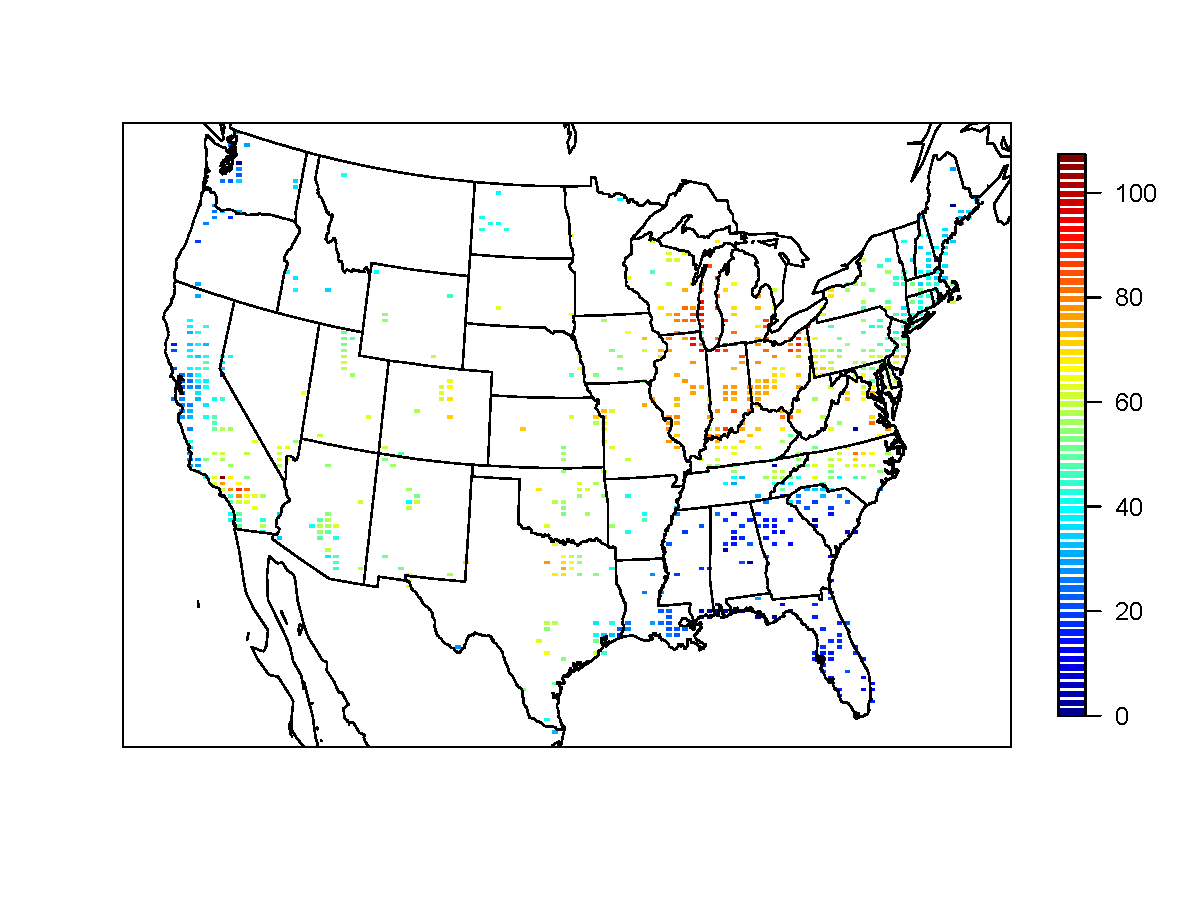
\includegraphics[width=\linewidth, trim=0 1in 0 1in ]{./plots/pot/ozone-10jul-us.pdf}
    \caption{Max 8-hour ozone measurements on July 10, 2005}
   \end{figure}
\end{frame}

\begin{frame}{Motivation}
  \begin{itemize} \setlength{\itemsep}{1em}
    \item Ozone compliance for Clean Air Act (EPA)
    \begin{itemize}
      \item Annual fourth-highest daily maximum 8-hour concentration, averaged over 3 years, not to exceed 75 ppb
      \item Annual fourth-highest is the 99th percentile for the year
      \item Common objectives are
      \begin{itemize}
        \item To interpolate to unmonitored sites
        \item Detect changes in extremes over time
        \item Study factors that lead to extreme events
      \end{itemize}
    \end{itemize}
  \end{itemize}
\end{frame}

\begin{frame}{Defining extremes}
\begin{columns}[c]
\column{.45 \linewidth}
  \begin{itemize} \setlength{\itemsep}{1em}
    \item Key in extreme value analysis is to define extremes
    \item Typically done in one of two ways
    \begin{itemize}
      \item Block maxima (red dots)
      \item Values over threshold considered extreme
    \end{itemize}
  \end{itemize}

  \column{.55\linewidth}
  \begin{figure}
    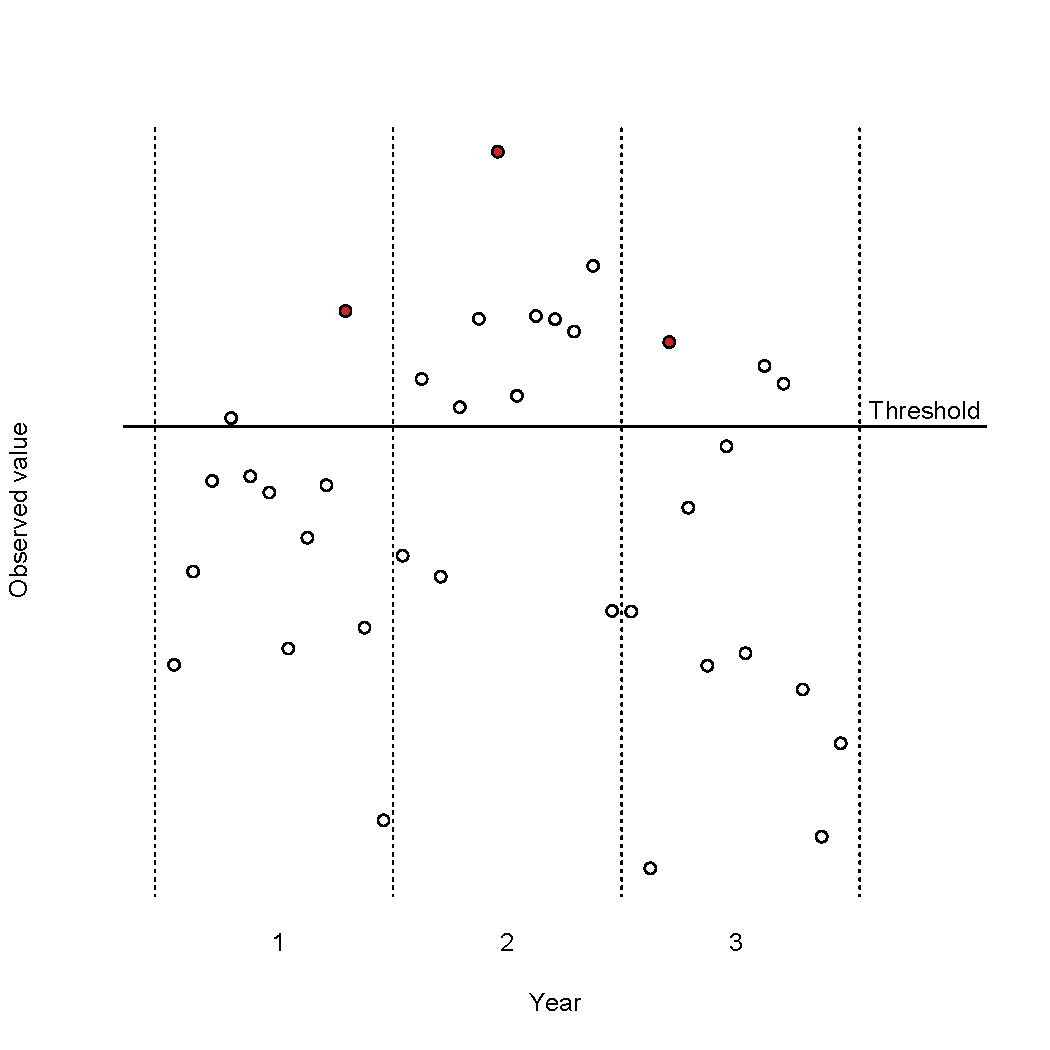
\includegraphics[width=1\linewidth, trim=0 0.5in 0 1in]{./plots/define_extreme.pdf}
    \caption{Hypothetical monthly maximums recorded over a three years}
    \end{figure}
\end{columns}
\end{frame}

\begin{frame}{Standard non-spatial analysis: Block maxima}
  \begin{itemize} \setlength{\itemsep}{1em}
    \item Let $X_1, \ldots, X_n$ be i.i.d.
    \item Consider the block maximum $M_n = \max(X_1, \ldots, X_n)$
    \item If there exist normalizing sequences $a_n > 0$ and $b_n \in \calR$ such that
    \begin{align*}
      \frac{ M_n - b_n }{ a_n } \converged G(z)
    \end{align*}
    then $G(z)$ follows a generalized extreme value distribution (GEV) (Falk et al., 2011)
    \item This motivates the use of the GEV for block max data
  \end{itemize}
\end{frame}

\begin{frame}{Standard non-spatial analysis: Block maxima}
  \begin{itemize} \setlength{\itemsep}{1em}
    \item GEV distribution
    \begin{align*}
      G(y) = \Pr(Y < y) = \left\{  \begin{array}{ll}
        \exp\left\{ -\left[ 1 + \xi \left( \frac{ y - \mu }{ \sigma } \right) \right]^{ -1 / \xi} \right\} & \quad \xi \neq 0 \\[0.5em]
        \exp \left\{ -\exp \left( - \frac{ y - \mu }{ \sigma} \right) \right\} & \quad \xi = 0
      \end{array}\right.
    \end{align*}
    where
    \begin{itemize}
      \item $\mu \in \calR$ is a location parameter
      \item $\sigma > 0$ is a scale parameter
      \item $\xi \in \calR$ is a shape parameter
      \begin{itemize}
        \item Unbounded above if $\xi \ge 0$
        \item Bounded above by $(\mu - \sigma) / \xi$ when $\xi < 0$
      \end{itemize}
    \end{itemize}
    \item Challenges:
    \begin{itemize}
      \item Lose information by only considering maximum in a block
      \item Underlying data may not be i.i.d.
    \end{itemize}
  \end{itemize}
\end{frame}

\begin{frame}{Standard non-spatial analysis: Peaks over threshold}
  \begin{itemize} \setlength{\itemsep}{1em}
    \item Let $X_1, \ldots, X_n \sim F$
    \item If there exist normalizing sequences $a_t > 0$ and $b_t \in \calR$ such that for any $x \ge 0$, as $T \rightarrow \infty$
    \begin{align*}
      \Pr\left(\frac{X - b_t}{a_t} > t \mid X > T\right) \converged H(x),
    \end{align*}
    where $T$ is a thresholding value, then $H(x)$ follows a generalized Pareto distribution (GPD) (Balkema and de Haan, 1974)
  \end{itemize}
\end{frame}

\begin{frame}{Standard non-spatial analysis: Peaks over threshold}
  \begin{itemize}  \setlength{\itemsep}{1em}
    \item Select a threshold, $T$, and use the Generalized Pareto distribution to model the exceedances
    \begin{align*}
      H(y) = P(Y < y) = \left\{ \begin{array}{ll}
        1 - \left[1 - \xi \left( \frac{ y - T }{ \sigma } \right) \right]^{-1 / \xi} & \quad \xi \neq 0 \\[0.5em]
        1 - \exp \left\{ \frac{ y - T }{ \sigma} \right\} & \quad \xi = 0
      \end{array}\right.
    \end{align*}
    where
    \begin{itemize}
      \item $\sigma > 0$ is a scale parameter
      \item $\xi \in \calR$ is a shape parameter
      \begin{itemize}
        \item Unbounded above if $\xi \ge 0$
        \item Bounded above by $(T - \sigma) / \xi$ when $\xi < 0$
      \end{itemize}
    \end{itemize}
  \end{itemize}
\end{frame}

\begin{frame}{Standard non-spatial analysis: Peaks over threshold}
  \begin{itemize} \setlength{\itemsep}{1em}
    \item The GPD is related to GEV distribution through
    \begin{align*}
      H(y) = 1 + \log[G(y)], \quad y \ge T
    \end{align*}
    \item Challenges:
    \begin{itemize}
      \item Sensitive to threshold selection
      \item Temporal dependence between observations (e.g. flood levels don't dissipate overnight)
    \end{itemize}
  \end{itemize}
\end{frame}


\begin{frame}{Max-stable processes for spatial data}
  \begin{itemize} \setlength{\itemsep}{1em}
    \item Consider i.i.d. spatial processes $x_j(\bs)$, $j = 1, \ldots, J$
    \item Let $M_J(\bs) = \bigvee_{j=1}^J x_j(\bs_i)$ be the block max at site $\bs$
    \item If there exists normalizing sequences $a_J(\bs)$ and $b_J(\bs)$ such that for all sites, $\bs_i, i = 1, \ldots, d$,
    \begin{align*}
      a_J^{-1}(\bs) \left\{ M_J(\bs) - b_J(\bs) \right\} \converged Y(\bs)
    \end{align*}
    which has a non-degenerate distribution, then $Y(\bs)$ is a max-stable process
    \item Therefore, max-stable processes are the standard for block maxima
  \end{itemize}
\end{frame}

\begin{frame}{Multivariate representations}
  \begin{itemize}
    \item Marginally at each site, observations follow a GEV distribution
    \item For a finite collection of sites the multivariate representation for the GEV (mGEV) is
    \begin{align*}
      \Pr(\bZ \le \bz)  &= G^*(\bz) = \exp(-V(\bz))\\
            V(\bz)    &= d \int_{\Delta_d} \bigvee_{i = 1}^d \frac{w_i}{z_i} H(\ddd w)
    \end{align*}
    where
    \begin{itemize}
      \item $\Delta_d = \{ \bw \in \calR^d_+ \mid w_1 + \cdots + w_d = 1\}$
      \item $H$ is a probability measure on $\Delta_d$
      \item $\int_{\Delta_d}w_i H(\ddd w) = 1 / d$ for $i = 1, \ldots, d$.
    \end{itemize}
  \end{itemize}
\end{frame}

\begin{frame}{Multivariate GEV challenges}
  \begin{itemize}
    \item Only a few closed-form expressions for $V(\bz)$ exist (Stephenson, 2003)
    \item Two common forms for $V(\bz)$:
    \begin{itemize}
      \item Symmetric logistic
      \begin{align*}
        V(\bz) = \left[\sum_{i = 1}^n \left( \frac{ 1 }{ z_i } \right)^{1/\alpha}\right]^\alpha
      \end{align*}
      \item Asymmetric logistic
      \begin{align*}
        V(\bz) = \sum_{l = 1}^L \left[\sum_{i = 1}^n \left(\frac{w_{il}}{z_i} \right)^{1 / \alpha_l} \right]^{\alpha_l}
      \end{align*}
      where $w_{il} \in [0, 1]$ and $\sum_{l = 1}^L w_{il} = 1$.
    \end{itemize}
  \end{itemize}
\end{frame}

\begin{frame}{Multivariate peaks over threshold}
  \begin{itemize}
    \item Few existing methods
    \item Often use max-stable methods due to the relationship between GEV and GPD
    \item Joint distribution function given by Falk et al. (2011)
    \begin{align*}
      H(\bz) = 1 - V(\bz)
    \end{align*}
    where $V(\bz)$ is defined as in the GEV
  \end{itemize}
\end{frame}

\begin{frame}{Extremal dependence: $\chi$ statistic}
  \begin{itemize} \setlength{\itemsep}{1em}
    \item Correlation is the most common measure of dependence
    \begin{itemize}
      \item Focuses on the center and not tails
      \item This makes it irrelevant for extreme value analysis
    \end{itemize}
    \item Extreme value analysis focuses on the $\chi$ statistic, a measure of extremal dependence given by
    \begin{align*}
      \chi(h) = \lim_{c \rightarrow \infty}\Pr[Y(\bs) > c \mid Y(\bt) > c]
    \end{align*}
    where $h = ||\bs - \bt||$
    \item If $ \chi(h) = 0$, then observations are asymptotically independent at distance $h$
  \end{itemize}
\end{frame}

\begin{frame}{Existing challenges}
  \begin{itemize} \setlength{\itemsep}{1em}
    \item Multivariate max-stable and GPD models have nice features, but they are
    \begin{itemize}
      \item Computationally challenging (e.g,  the asymmetric logistic has $2^{n-1}(n + 2) - (2n + 1)$ free parameters)
      \item Joint distribution only available in low dimensions
    \end{itemize}
    \item Some recent approaches
    \begin{itemize}
      \item Bayesian hierarchical model (Reich and Shaby, 2012)
      \item Pairwise likelihood approach (Huser and Davison, 2014)
    \end{itemize}
    \item Many opportunities to explore new methods
  \end{itemize}
\end{frame}

\begin{frame}{Three principal contributions}
  \begin{enumerate}[1] \setlength{\itemsep}{1em}
    \item A spatio-temporal model with flexible tails, asymptotic spatial dependence, and computation on the order of Gaussian models for large space-time datasets
    \item Predicting rare binary events with a spatially dependent generalized extreme-value link function
    \item A Bayesian hierarchical model to allow for non-stationary covariance in extreme value models
  \end{enumerate}
\end{frame}

\begin{frame}{Spatiotemporal modeling for extreme values}
  \begin{itemize} \setlength{\itemsep}{1em}
    \item Model objectives:
    \begin{itemize}
      \item Marginal distribution with a flexible tail
      \begin{itemize}
        \item Allow for asymmetric distributions
        \item Allow for heavy tails
      \end{itemize}
      \item Asymptotic spatial dependence
      \item Computation on the order of Gaussian models for large space-time datasets
    \end{itemize}
  \end{itemize}
\end{frame}

\begin{frame}{Gaussian spatial model}
  \begin{itemize} \setlength{\itemsep}{1em}
    \item In geostatistics $Y(\bs)$ are often modeled using a Gaussian process with mean function $\mu(\bs)$ and covariance function $\rho(h)$.
    \item Model properties
    \begin{itemize}
      \item Nice computing properties (closed-form likelihood)
      \item For a Gaussian spatial model $\lim_{c \rightarrow \infty} \chi(h) = 0$ regardless of the strength of the correlation in the bulk of the distribution
      \item Tail is not flexible
      \begin{itemize}
        \item Light-tailed
        \item Symmetric
      \end{itemize}
    \end{itemize}
  \end{itemize}
\end{frame}

\begin{frame}{Spatial skew-$t$ distribution}
  \begin{itemize} \setlength{\itemsep}{1em}
    \item A more flexible alternative is the spatial skew-$t$ process (Zhang and El-Shaarawi, 2012)
    \begin{align*}
      Y(\bs) = \bX(\bs)\bbeta + \lambda |z| + v(\bs)
    \end{align*}
    where
    \begin{itemize} \setlength{\itemsep}{0.25em}
      \item $\lambda \in \calR$ controls the skewness
      \item $z \sim N(0, \sigma^2)$ is a random effect
      \item $v(\bs)$ is a Gaussian process with variance $\sigma^2$ and \Matern correlation
      \item $\sigma^2 \sim \text{IG}(a, b)$
    \end{itemize}
  \end{itemize}
\end{frame}

\begin{frame}{Spatial skew-$t$ distribution}
  \begin{itemize} \setlength{\itemsep}{1em}
    \item \alert{Conditioned} on $z$ and $\sigma^2$, $Y(\bs)$ is a Gaussian spatial model
    \item Can use standard geostatistical methods to fit this model
    \item Predictions can be made through Kriging
  \end{itemize}
\end{frame}

\begin{frame}{Spatial skew-$t$ distribution}
  \begin{itemize} \setlength{\itemsep}{1em}
    \item \alert{Marginalizing} over $z$ and $\sigma^2$ (via MCMC),
    \begin{align*}
      Y(\bs) \sim \text{skew-t}(\bX(\bs), \bOmega, \alpha, \text{df}=2a)
    \end{align*}
    where
    \begin{itemize}
      \item $\bX(\bs) \bbeta$ is the location
      \item $\bOmega = \frac{1}{ab} \bar{\bOmega}$ is a correlation matrix
      \item $\bar{\bOmega} = (\bSigma + \lambda^2 \bOne \bOne^T)$
      \item $\bSigma$ is a postive definite correlation matrix
      \item $\alpha = \lambda( 1 + \lambda^2 \bOne^T \bSigma^{-1} \bOne)^{-1/2} \bOne^T \bSigma^{-1}$ controls the skewness
    \end{itemize}
  \end{itemize}
\end{frame}

\begin{frame}{$\chi(h)$ plot}
  \vspace{-2em}
  \centering
  \begin{figure}
  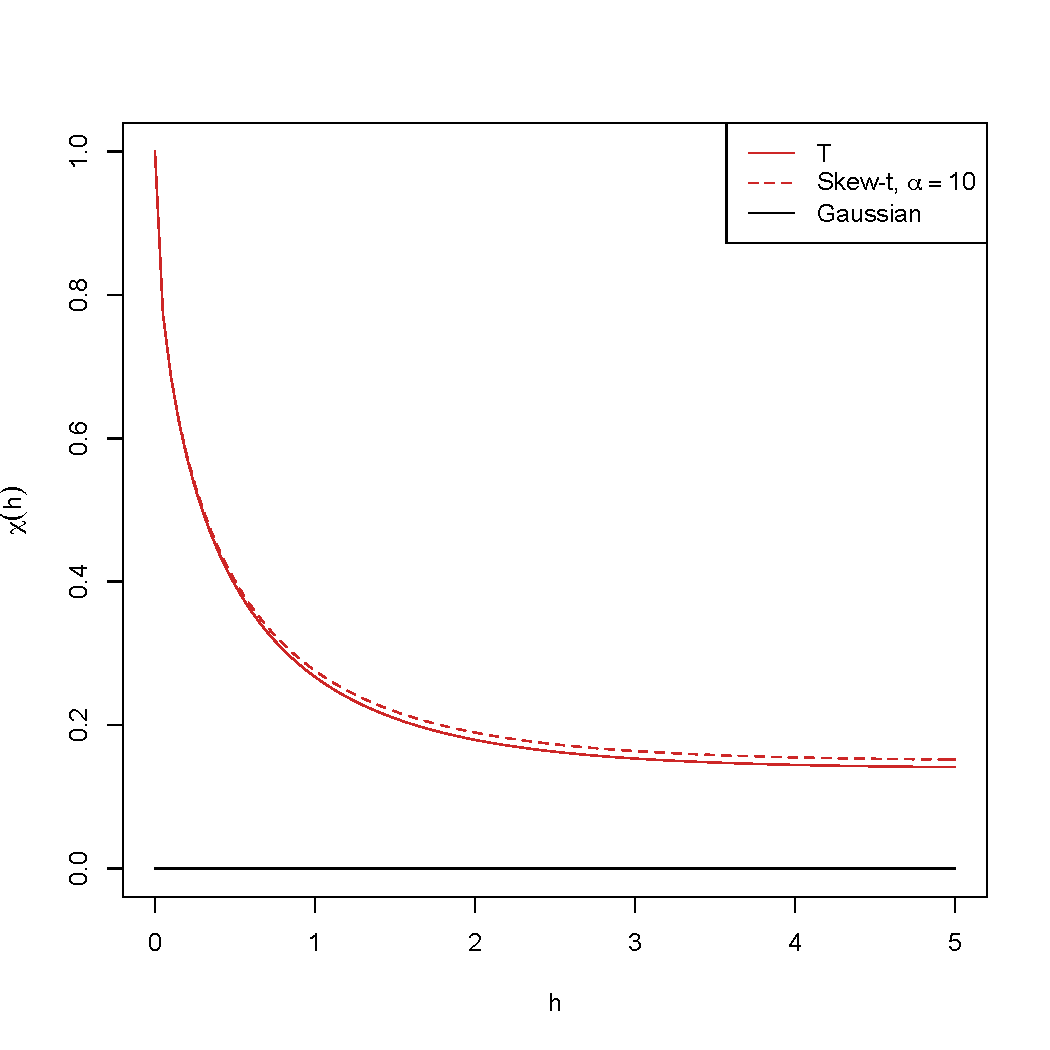
\includegraphics[width=.65\linewidth]{./plots/pot/chi-h-t_and_gaus.pdf}\\[-0.2in]
  \caption{$\chi$ plot for skew-$t$, and Gaussian}
  \end{figure}
\end{frame}

\begin{frame}{Spatial skew-$t$ distribution properties}
  \begin{itemize} \setlength{\itemsep}{1em}
    \item Model properties:
    \begin{itemize}
      \item Flexible tail
      \begin{itemize}
        \item Skewness controlled by $\lambda$
        \item Weight of tails controlled by degrees of freedom $2a$
      \end{itemize}
      \item For a skew-$t$ distribution $\lim_{c \rightarrow \infty} \chi(h) > 0$ (Padoan, 2011)
      \item Computation that is on the order of Gaussian computation
    \end{itemize}
    \item Challenge: $\chi(h) > 0$ as $h \rightarrow \infty$ (Padoan, 2011)
    \begin{itemize}
      \item This occurs because all observations (near and far) share the same $z$ and $\sigma^2$
    \end{itemize}
  \end{itemize}
\end{frame}

\begin{frame}{Extension of the skew-$t$ distribution}
  \begin{itemize} \setlength{\itemsep}{1em}
    \item Skew-$t$ distribution addresses two modeling concerns
    \begin{itemize}
      \item Extremal dependence
      \item Reasonable computing
    \end{itemize}
    \item Our contribution is to extend the skew-$t$
    \begin{itemize}
      \item Censoring to focus on extreme observations
      \item Partitioning to address long-range dependence
    \end{itemize}
  \end{itemize}
\end{frame}

\begin{frame}{Censoring data to focus on tail behavior}
  \begin{itemize} \setlength{\itemsep}{1em}
    \item We censor the observed data at a high threshold $T$
    \item Censored data
    \begin{align*}
      \tilde{Y}_t(\bs) = \left\{ \begin{array}{ll}
          Y_t(\bs) \quad & \delta(\bs) = 1\\
          T \quad & \delta(\bs) = 0
      \end{array}\right.
    \end{align*}
    where $\delta(\bs) = I[Y(\bs) > T]$
    \item Allows tails of the distribution to speak for themselves
  \end{itemize}
\end{frame}

\begin{frame}{Random partition}
  \begin{itemize} \setlength{\itemsep}{1em}
    \item Daily random partition allows $z$ and $\sigma^2$ to vary by site
    \begin{align*}
      Y(\bs) = \bX(\bs) \bbeta + \lambda z(\bs) + \sigma(\bs) v(\bs)
    \end{align*}
    \item Consider a set of knots $\bw_{k} \sim$ Uniform that define a random partition
    $P_{1}, \ldots, P_{K}$ such that
    \begin{align*}
      P_{k} = \{s : k = \argmin_\ell|| \bs - \bw_{\ell}|| \}
    \end{align*}
    where $\bw = (w_1, w_2)$ (similar to Kim et al., 2005 for non-extreme modeling)
    \item For $\bs \in P_{k}$
    \begin{align*}
      z(\bs) &= z_{k}\\
      \sigma^2(\bs) &= \sigma^2_{k}
    \end{align*}
  \end{itemize}
\end{frame}

\begin{frame}{Example partition}
    \centering
    \begin{figure}
    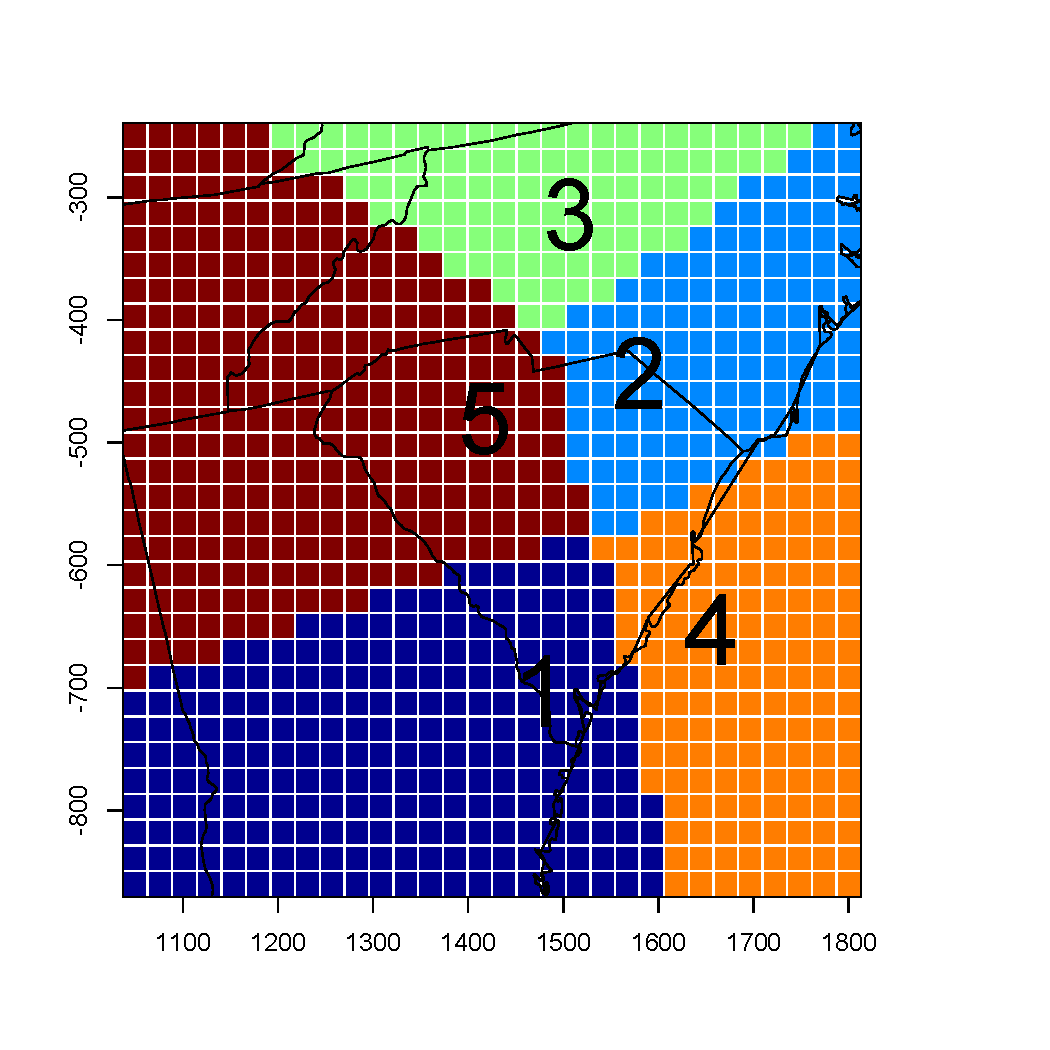
\includegraphics[width=0.54\linewidth, trim=0 0 0 1in]{./plots/pot/example-partition-1.pdf}
    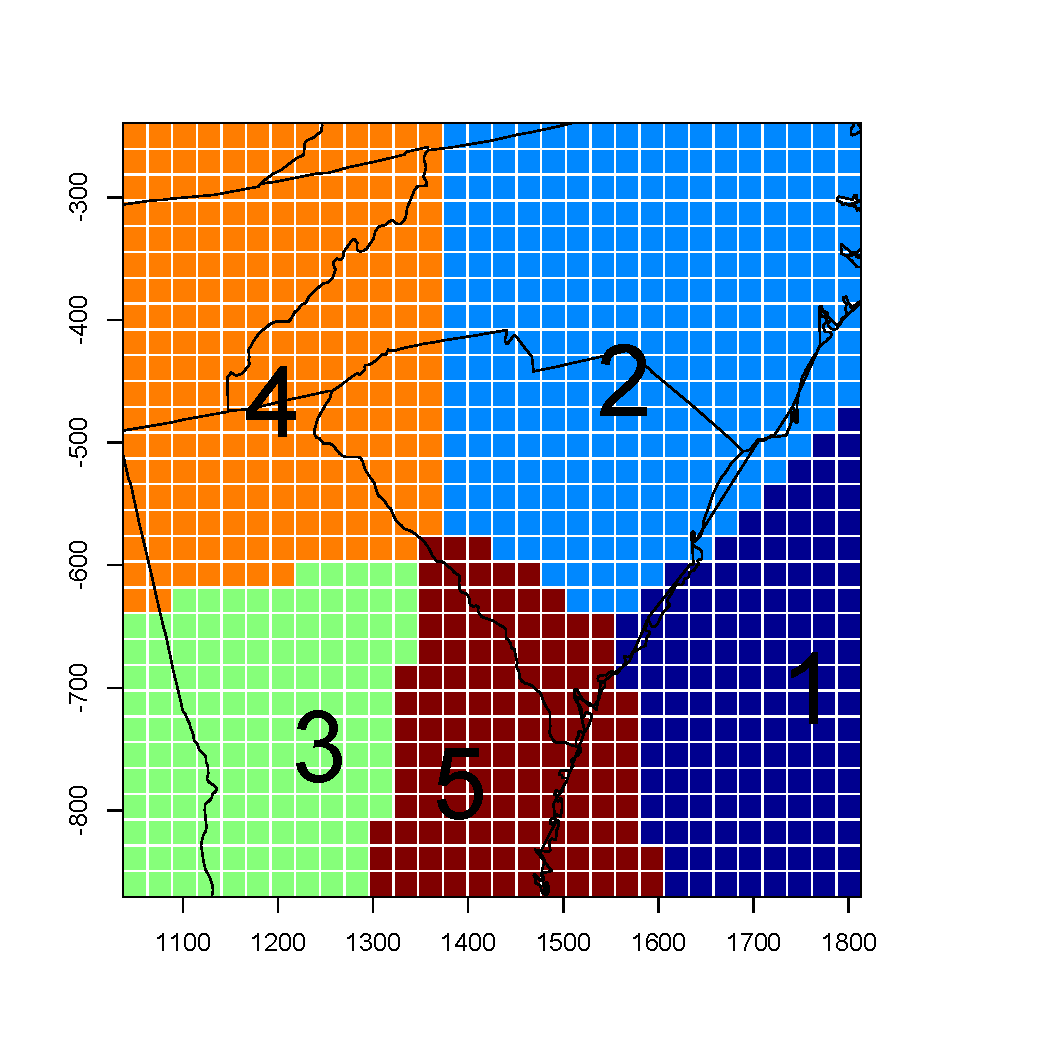
\includegraphics[width=0.54\linewidth, trim=0 0 0 1in]{./plots/pot/example-partition-2.pdf}
    \caption{Two sample partitions (number is at partition center)}
    \end{figure}
\end{frame}

\begin{frame}{Random partition}
  \begin{itemize} \setlength{\itemsep}{1em}
    \item Within each partition $Y(\bs)$ has the same MV skew-t distribution as before
    \item Across partitions $Y(\bs)$ are asymptotically independent, but still correlated through $v(\bs)$
    \item New expression for $\chi(h)$
    \begin{align*}
      \chi(h) = \pi(h) \chi_{\text{skew-}t}(h)
    \end{align*}
    where
    \begin{itemize}
      \item $\pi(h)$ is the probability two sites are in the same partition
    \end{itemize}
  \end{itemize}
\end{frame}

\begin{frame}{$\chi(h)$ plot}
  \vspace{-2em}
  \centering
  \begin{figure}
  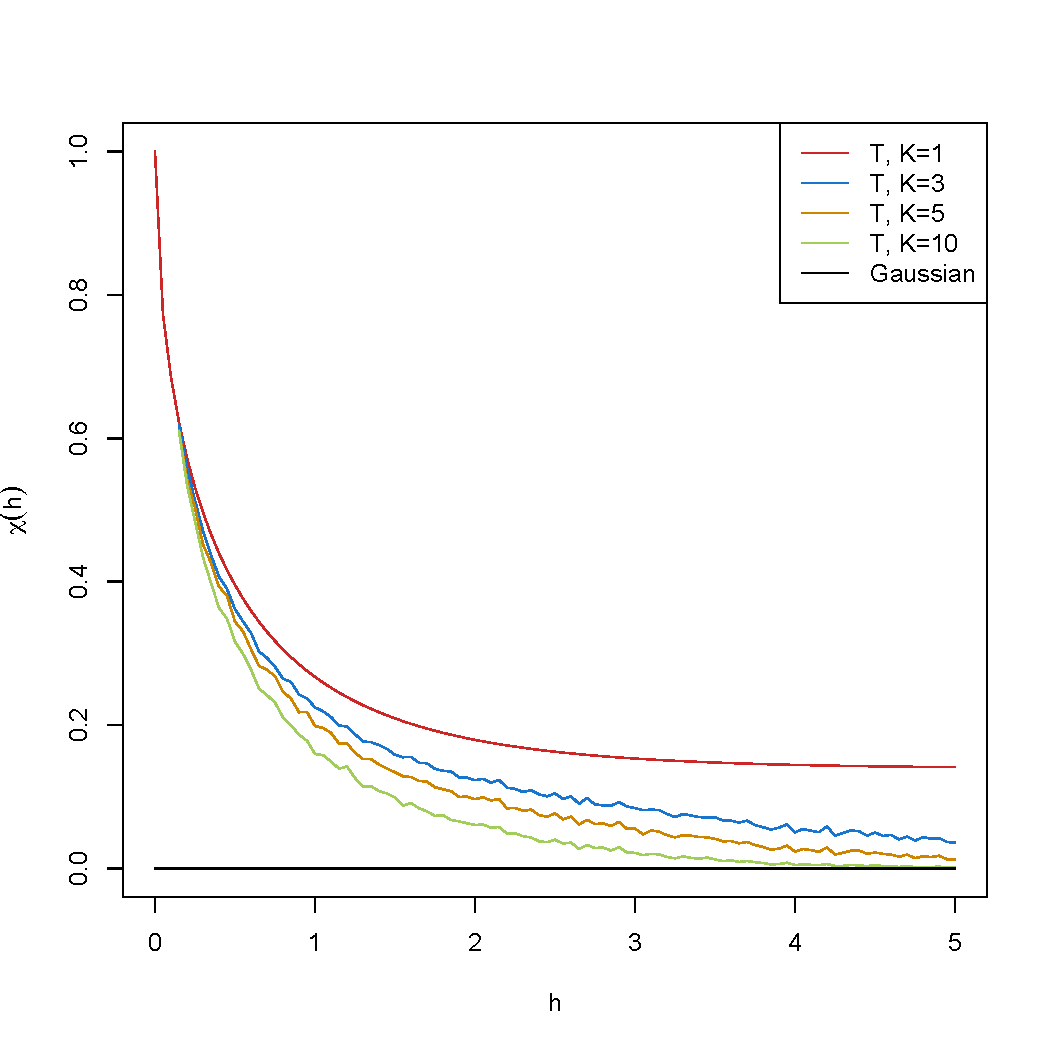
\includegraphics[width=.65\linewidth]{./plots/pot/chi-h.pdf}\\[-0.2in]
  \caption{$\chi$ plot for different data settings}
  \end{figure}
\end{frame}

\begin{frame}{Random partition skew-$t$ model}
  \begin{itemize} \setlength{\itemsep}{1em}
    \item This new model is called a random partition skew-$t$ model, and it has the properties we desire
    \begin{itemize}
      \item Marginal distribution with flexible tails
      \begin{itemize}
        \item $\lambda$ term allows for asymmetry
        \item Degrees of freedom control heavy vs light tails
      \end{itemize}
      \item Asymptotic spatial dependence for that decays with distance between sites through partitioning
      \item Computation is on the order of Gaussian models for large space-time datasets
    \end{itemize}
  \end{itemize}
\end{frame}

% \begin{frame}{Sample simulated datasets}
%   \centering
%   \begin{figure}
%   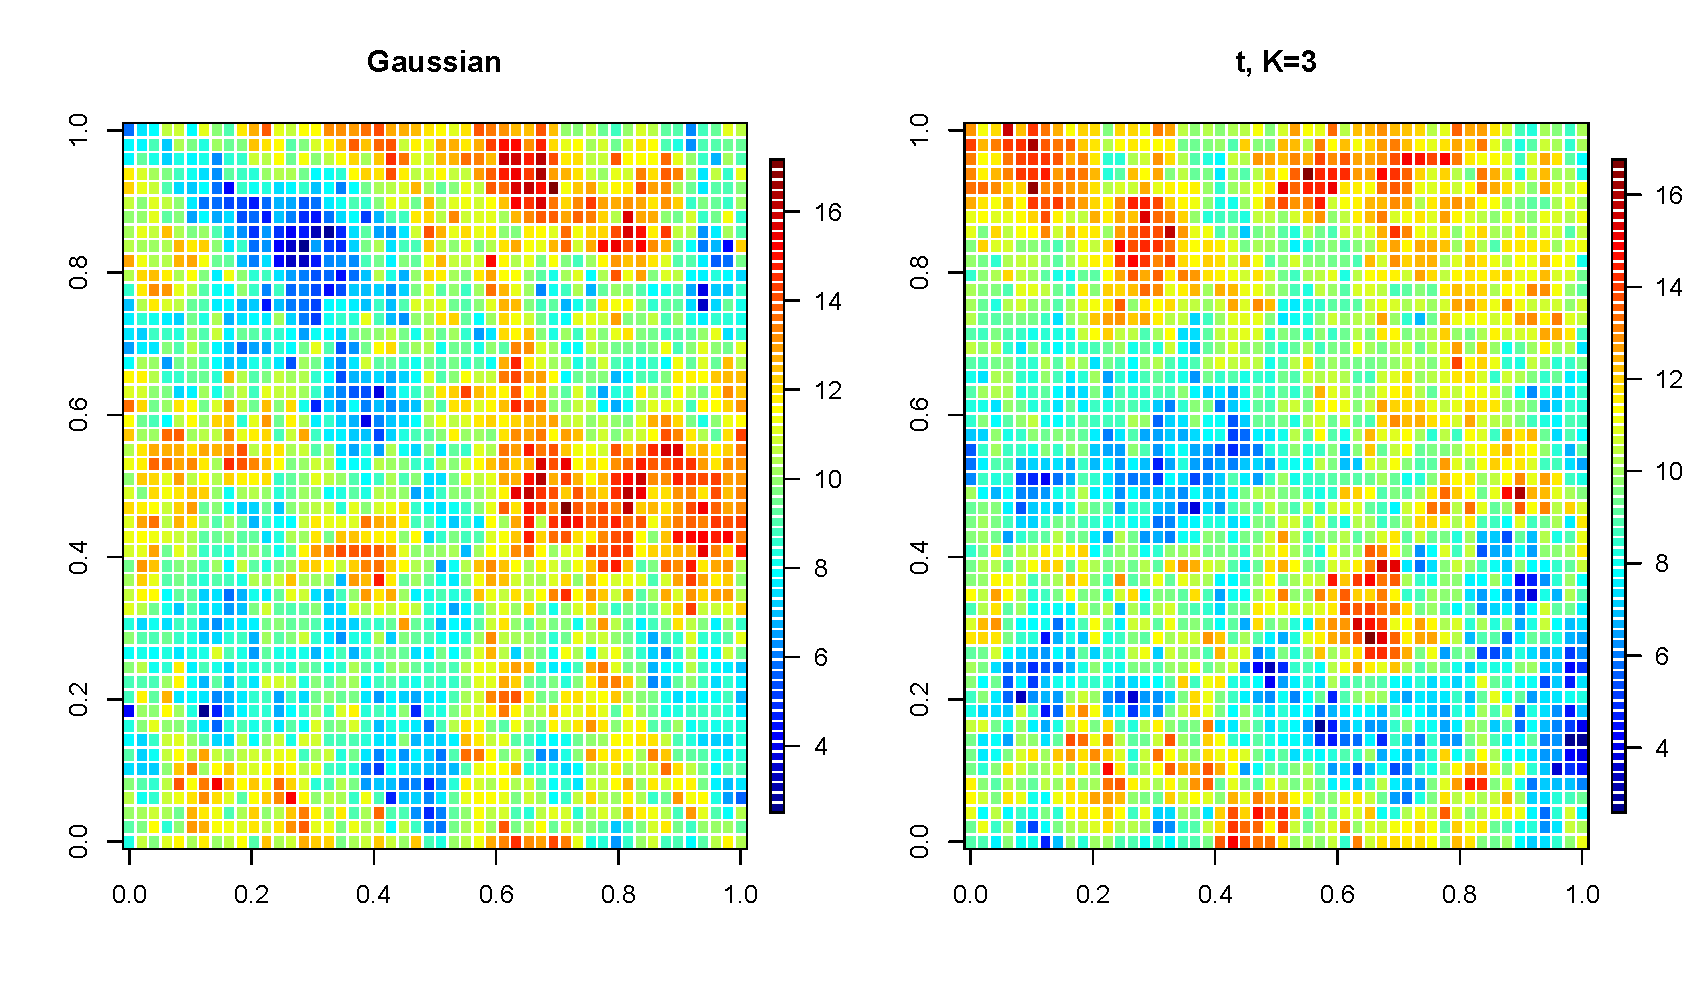
\includegraphics[width=1\linewidth]{./plots/pot/gauss-vs-t3.pdf}
%   \caption{Gaussian and $t$ with 3 partitions}
%   \end{figure}
% \end{frame}

% \begin{frame}{Sample simulated datasets}
%   \centering
%   \begin{figure}
%   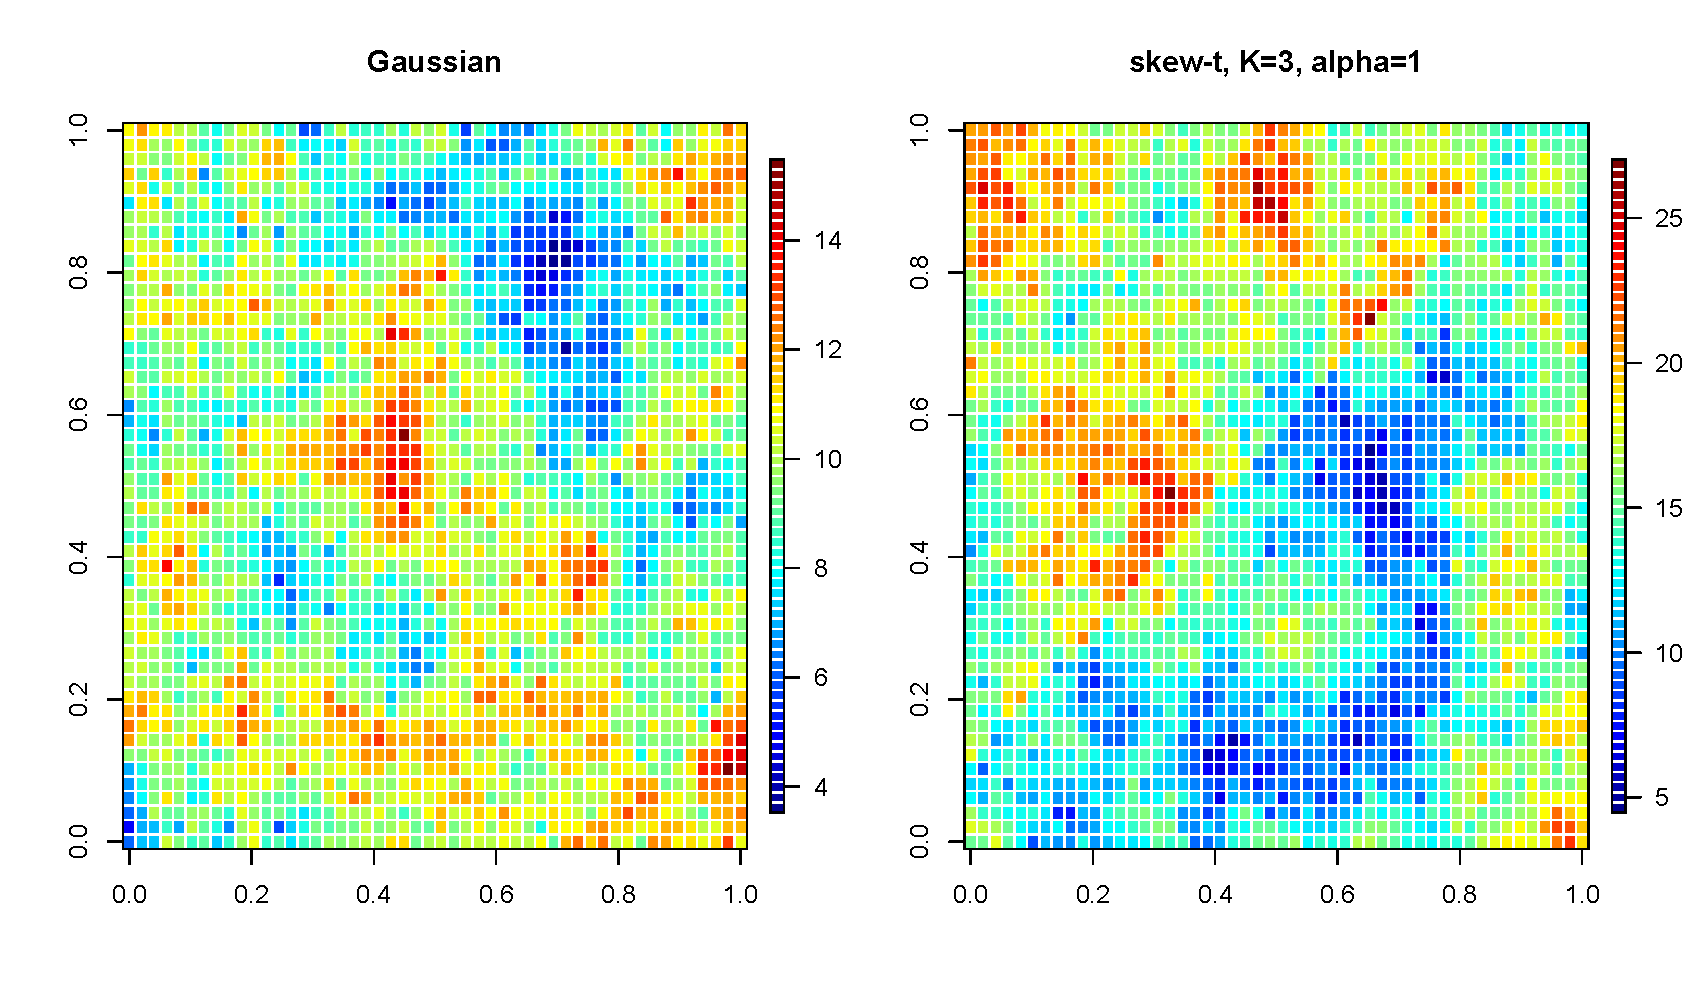
\includegraphics[width=1\linewidth]{./plots/pot/gauss-vs-skew-t3.pdf}
%   \caption{Gaussian and skew-$t$ with 3 partitions}
%   \end{figure}
% \end{frame}


\begin{frame}{MCMC details}
  \begin{itemize} \setlength{\itemsep}{1em}
    \item Three main steps
    \begin{enumerate}[1.]
      \item Impute censored data below $T$
      \item Update parameters with standard random walk Metropolis Hastings or Gibbs sampling
      \item Make spatial predictions
    \end{enumerate}
    \item Priors are selected to be conjugate when possible
  \end{itemize}
\end{frame}

\begin{frame}{Simulation study}
  \begin{itemize} \setlength{\itemsep}{1em}
    \item 6 different data settings
    \begin{itemize}
      \item Gaussian, $K = 1$ partition
      \item Symmetric-$t$, $K = 1$ partition
      \item Symmetric-$t$, $K = 5$ partitions
      \item Skew-$t$, $K = 1$ partition
      \item Skew-$t$, $K = 5$ partitions
      \item Max-stable
      \begin{itemize}
        \item Marginally: GEV$(\mu=1, \sigma=1, \xi=0.2)$
        \item Dependence function: asymmetric logistic with $\alpha = 0.5$
      \end{itemize}
    \end{itemize}
  \end{itemize}
\end{frame}

\begin{frame}{Simulation study}
  \begin{itemize} \setlength{\itemsep}{1em}
    \item 50 datasets for each setting
    \begin{itemize}
      \item 144 sites in $[0, 10] \times [0, 10]$
      \begin{itemize}
        \item 100 training
        \item 44 testing
      \end{itemize}
    \end{itemize}
    \item Model parameters
    \begin{itemize}
      \item Spatial range: $\rho = 1$
      \item Skew parameter: $\lambda = 3$
      \item Degrees of freedom: 6 for $t$ distributions
    \end{itemize}
  \end{itemize}
\end{frame}

\begin{frame}{Simulation study}
  \begin{itemize} \setlength{\itemsep}{1em}
    \item 5 different models fit to each data set
    \begin{itemize}
      \item Gaussian
      \item Skew-$t$ with $K = 1$ partition, no thresholding
      \item Skew-$t$ with $K = 1$ partition, thresholding at $q(0.80)$
      \item Skew-$t$ with $K = 5$ partitions, no thresholding
      \item Skew-$t$ with $K = 5$ partitions, thresholding at $q(0.80)$
    \end{itemize}
  \end{itemize}
\end{frame}

% \begin{frame}{Quantile score for cross-validation}
%   \begin{itemize} \setlength{\itemsep}{1em}
%     \item The quantile score for the $\tau$th quantile is
%     \begin{align*}
%       2 \{ I[y < \widehat{q}(\tau)] - \tau\} (\widehat{q} - y)
%     \end{align*}
%     where:
%     \begin{itemize}
%       \item $y$ is a test set value
%       \item $\widehat{q}(\tau)$ is the estimated $\tau$th quantile
%     \end{itemize}
%   \end{itemize}
% \end{frame}

\begin{frame}{Brier score}
  \begin{itemize} \setlength{\itemsep}{1em}
    \item Brier score used to determine model that gives best fit (Gneiting and Raftery, 2007)
    \item The Brier score for predicting exceedance of threshold $c$ is
    \begin{align*}
      [e(c) - P(c)]^2
    \end{align*}
    where
    \begin{itemize}
      \item $y$ is a test set value
      \item $e(c) = I[y > c]$
      \item $P(c)$ is the predicted probability of exceeding $c$
    \end{itemize}
    \item Relative Brier scores:
    \begin{align*}
      \text{BS}_\text{rel} = \frac{ \text{BS}_\text{method}}{ \text{BS}_\text{Gaussian}}
    \end{align*}
  \end{itemize}
\end{frame}

\begin{frame}{Simulation study results}
\centering
  \begin{figure}
    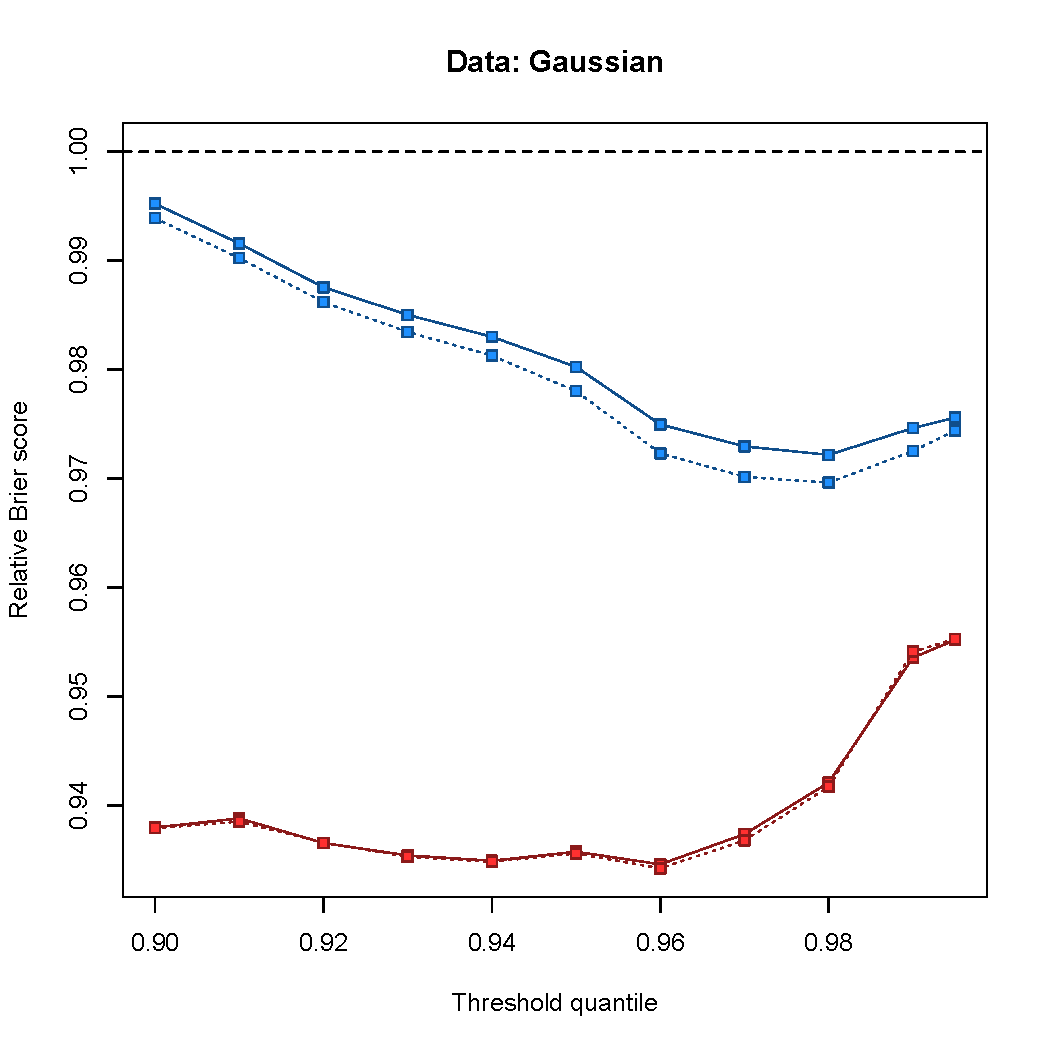
\includegraphics[width=0.45\linewidth]{./plots/pot/bs-sim-gaus.pdf}
    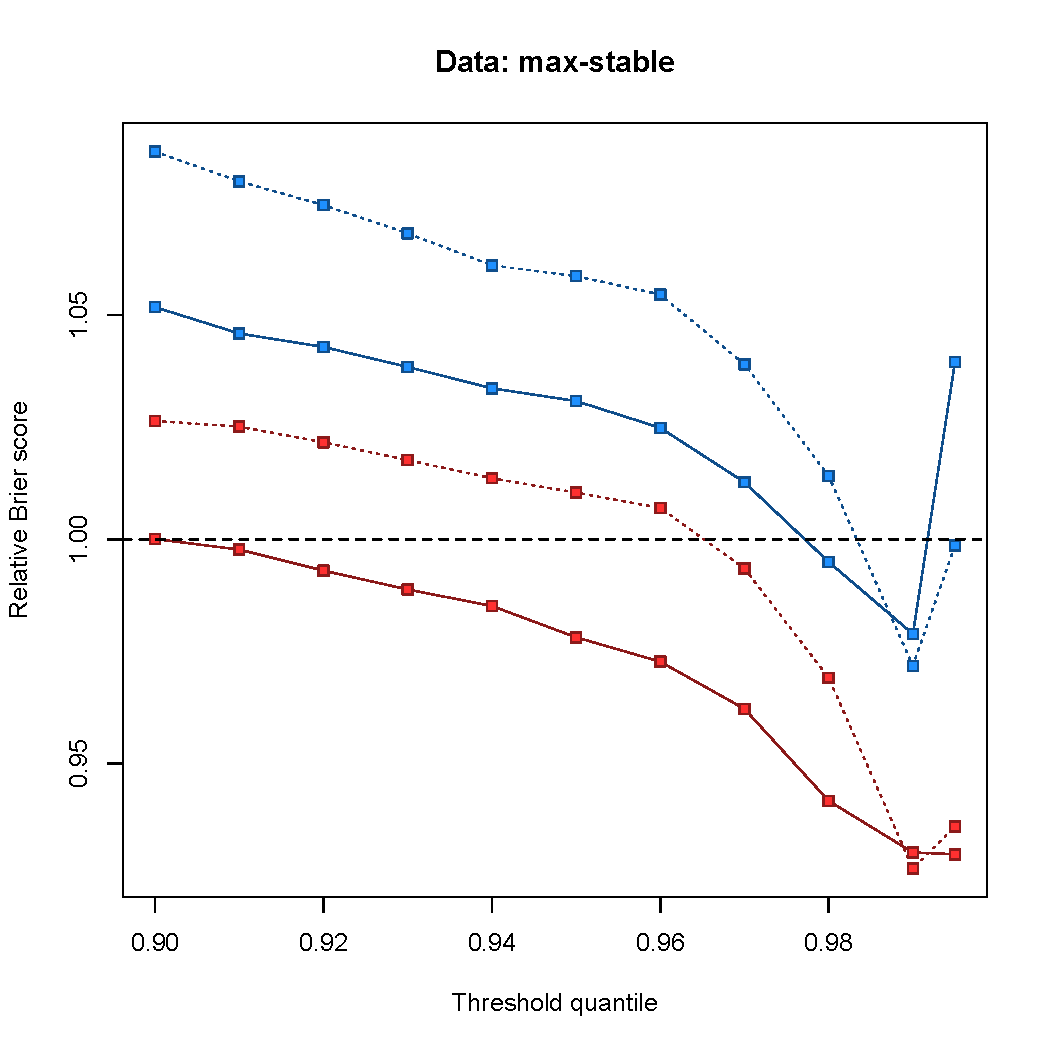
\includegraphics[width=0.45\linewidth]{./plots/pot/bs-sim-max.pdf} \\
    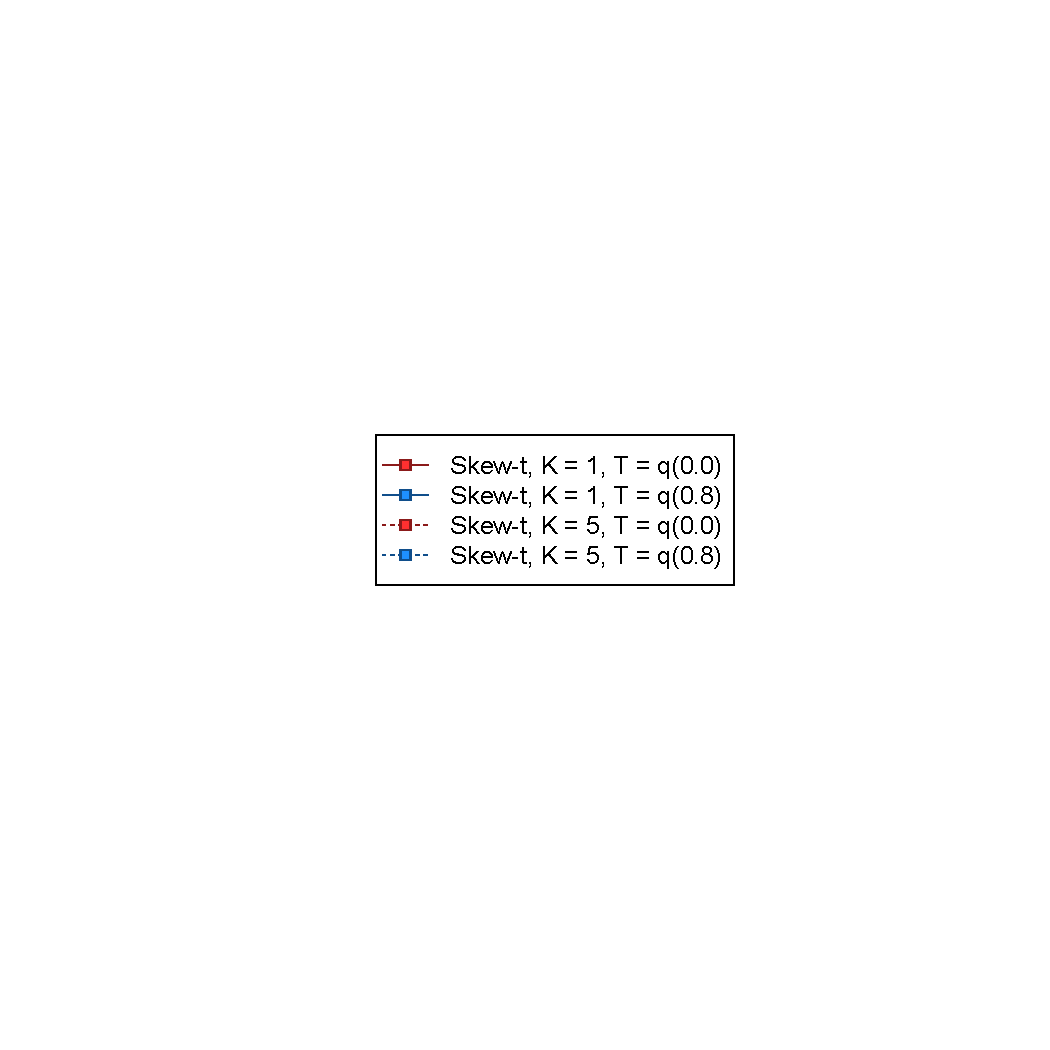
\includegraphics[width=0.3\linewidth, trim=2in 3.25in 2in 3in]{./plots/pot/bs-sim-legend.pdf}
    \caption{Relative Brier score results}
  \end{figure}
\end{frame}

\begin{frame}{Simulation study results}
\centering
  \begin{figure}
    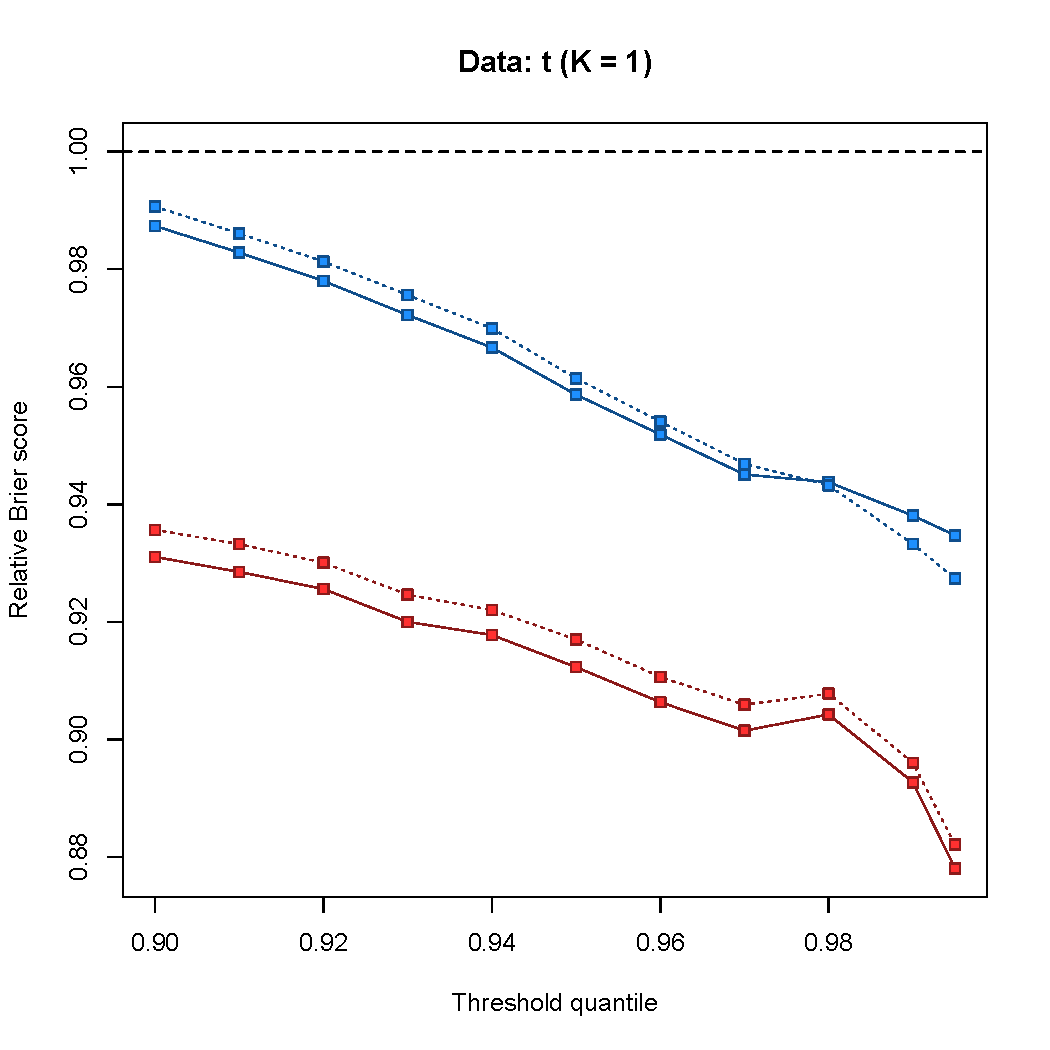
\includegraphics[width=0.45\linewidth]{./plots/pot/bs-sim-t1.pdf}
    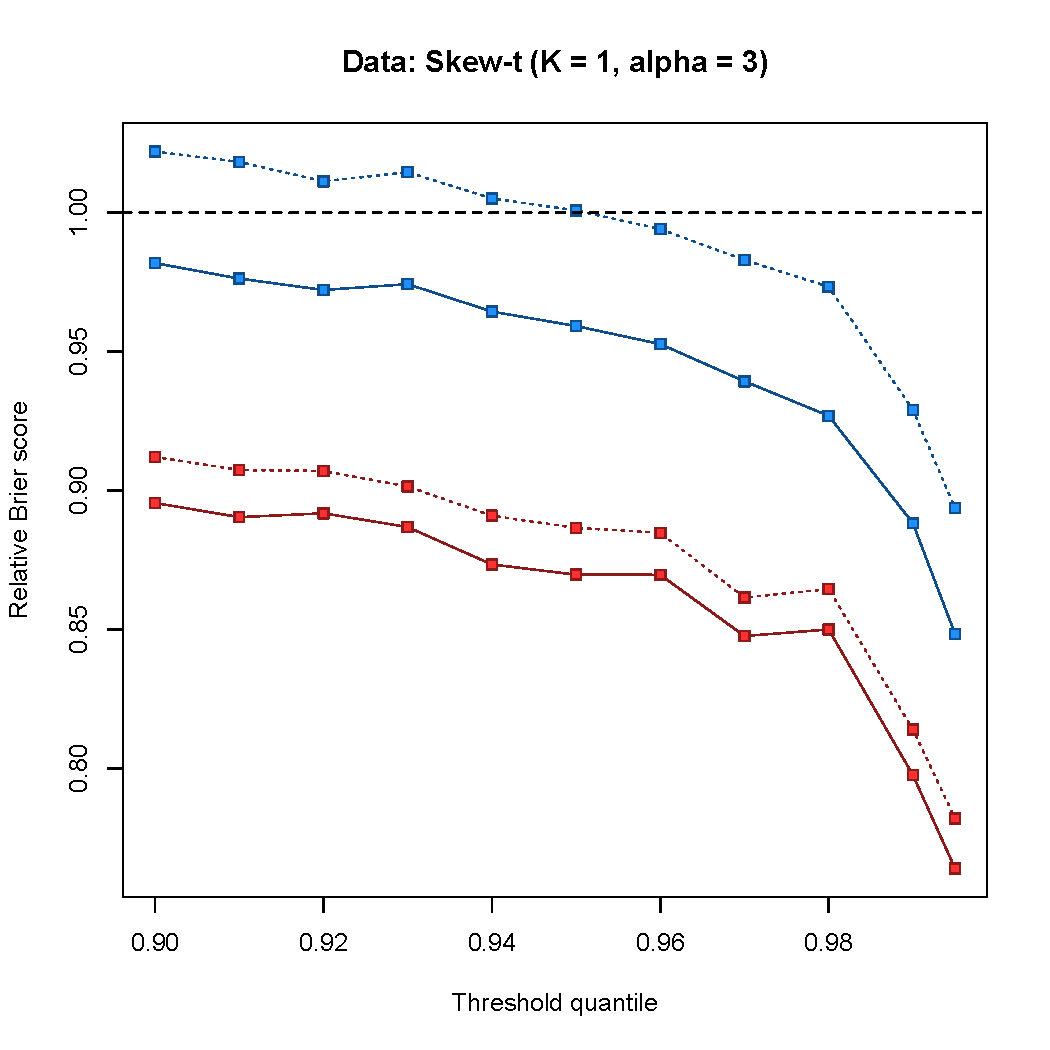
\includegraphics[width=0.45\linewidth]{./plots/pot/bs-sim-st1.pdf} \\
    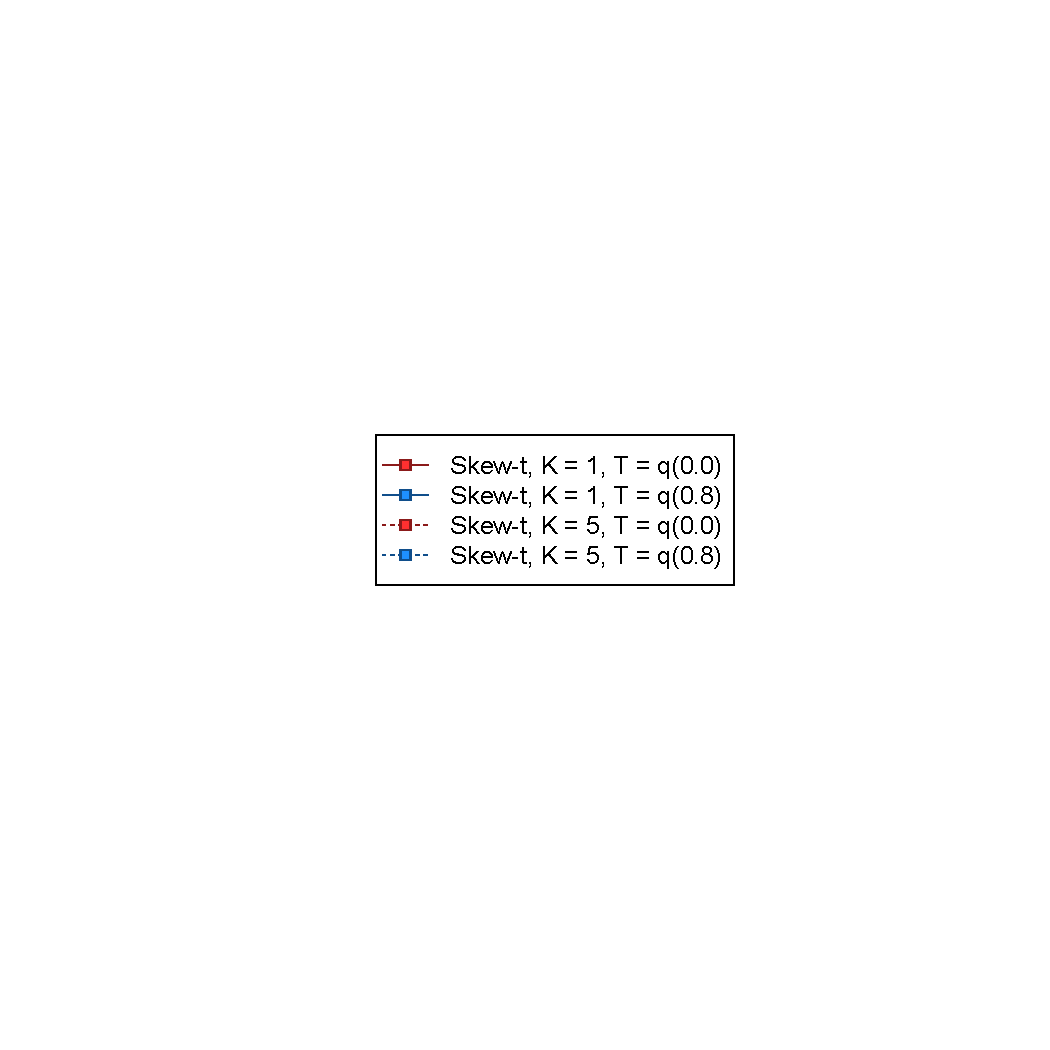
\includegraphics[width=0.3\linewidth, trim=2in 3.25in 2in 3in]{./plots/pot/bs-sim-legend.pdf}
    \caption{Relative Brier score results}
  \end{figure}
\end{frame}

\begin{frame}{Simulation study results}
\centering
  \begin{figure}
    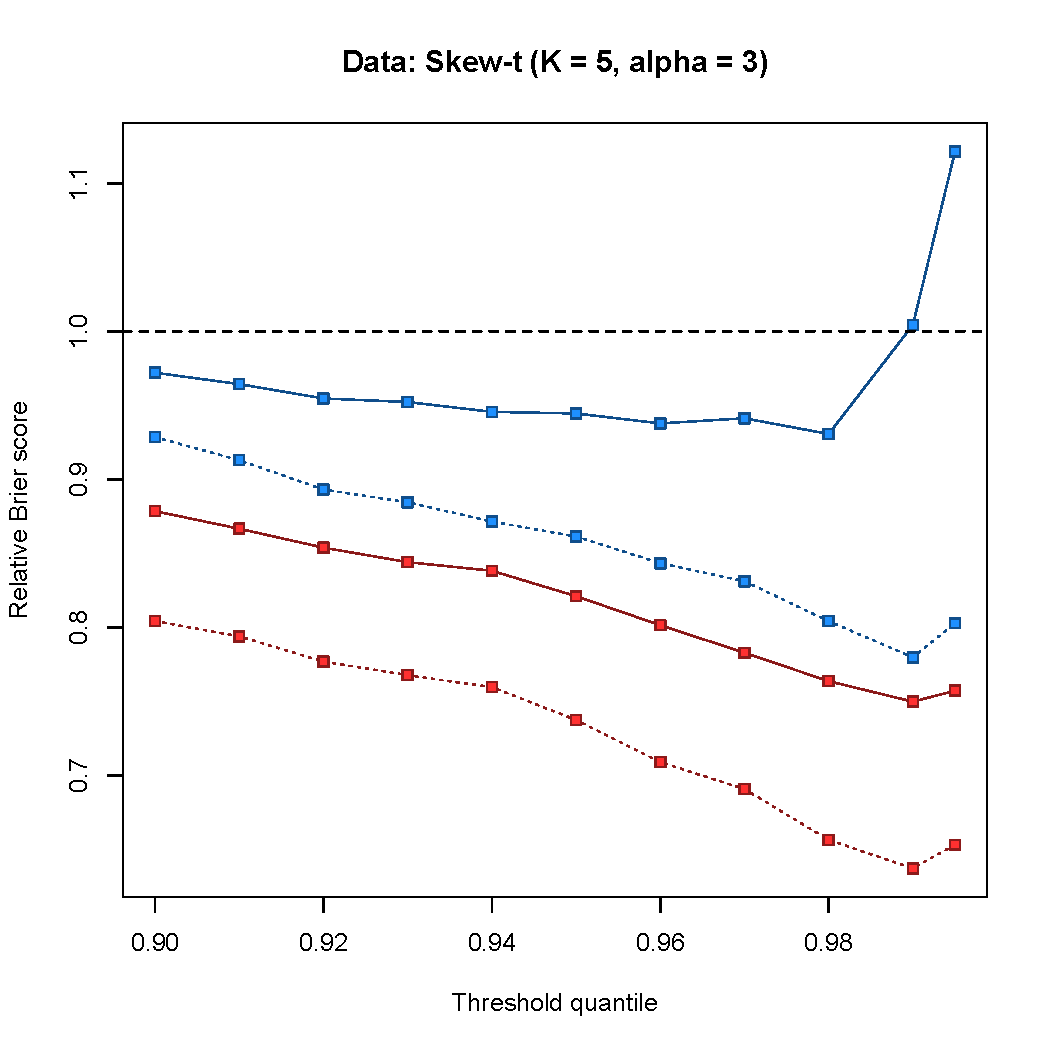
\includegraphics[width=0.45\linewidth]{./plots/pot/bs-sim-t5.pdf}
    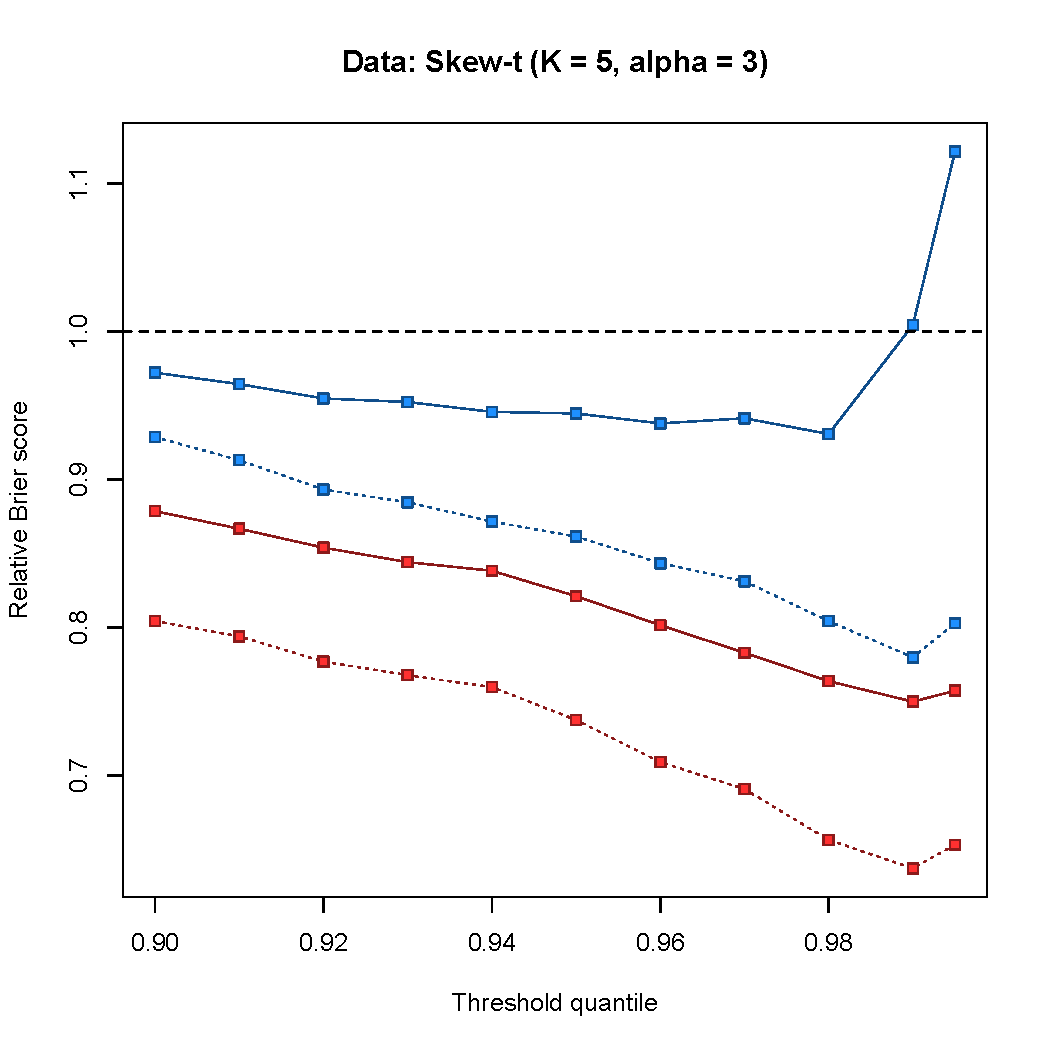
\includegraphics[width=0.45\linewidth]{./plots/pot/bs-sim-st5.pdf} \\
    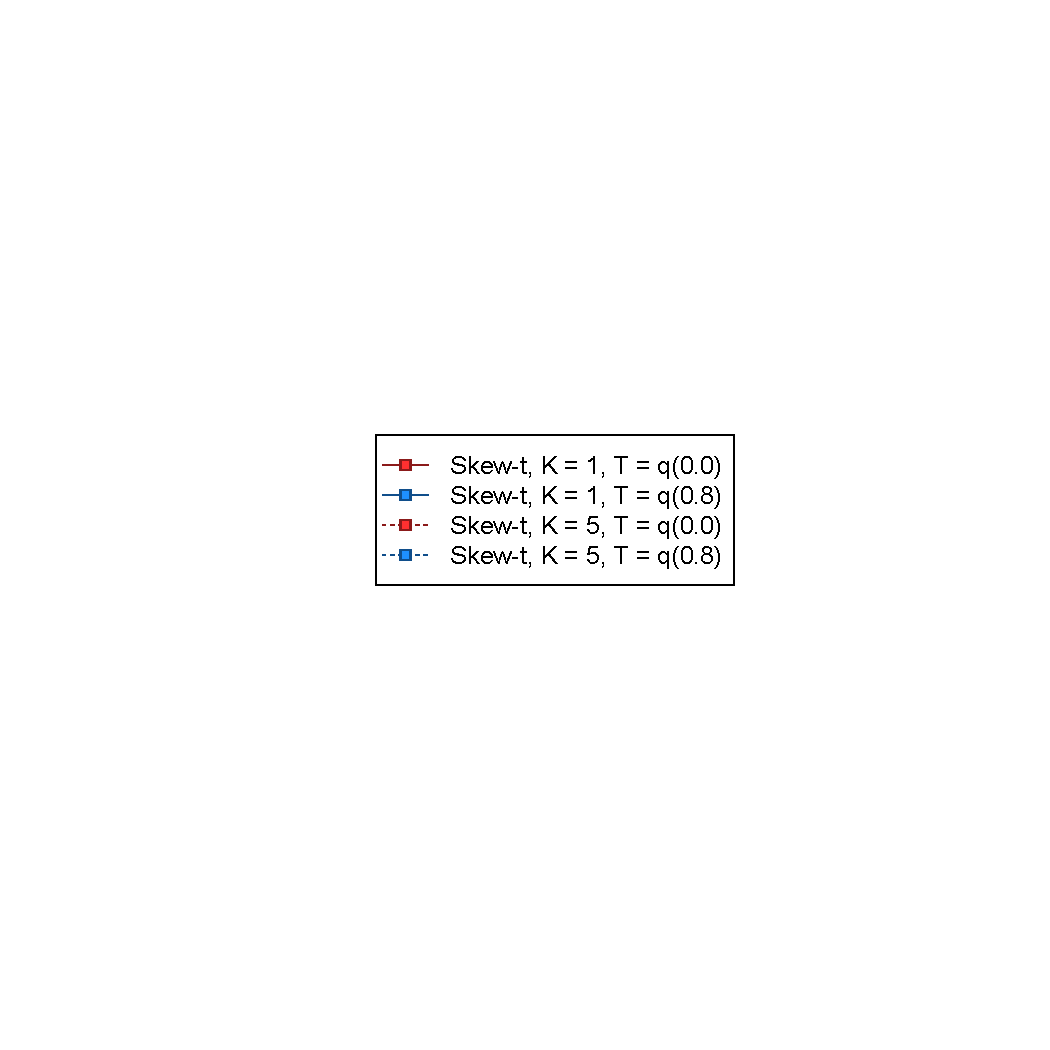
\includegraphics[width=0.3\linewidth, trim=2in 3.25in 2in 3in]{./plots/pot/bs-sim-legend.pdf}
    \caption{Relative Brier score results}
  \end{figure}
\end{frame}

\begin{frame}{Simulation study results}
  \begin{itemize} \setlength{\itemsep}{1em}
    \item Key findings
    \begin{itemize}
      \item Improvement over Gaussian methods when partitioning
      \item Specifying too few knots has a detrimental impact
      \item In all cases, non-thresholded models perform better than thresholded models
    \end{itemize}
  \end{itemize}
\end{frame}

\begin{frame}{Data analysis}
\begin{columns}[c]
\column{.45 \linewidth}
	\begin{itemize} \setlength{\itemsep}{1em}
	\item Ozone measurements
	\begin{itemize}
		\item max 8-hour ozone measurements
		\item daily data from 1089 sites
		\item July 2005
	\end{itemize}
  \item We take a stratified sample of $n = 800$ sites
  \begin{itemize}
    \item 271 from northeast
    \item 96 from northwest
    \item 269 from southeast
    \item 164 from southwest
  \end{itemize}
  \item Conduct two-fold cross-validation on 800 sites
	\end{itemize}

	\column{.55\linewidth}
	\begin{figure}
    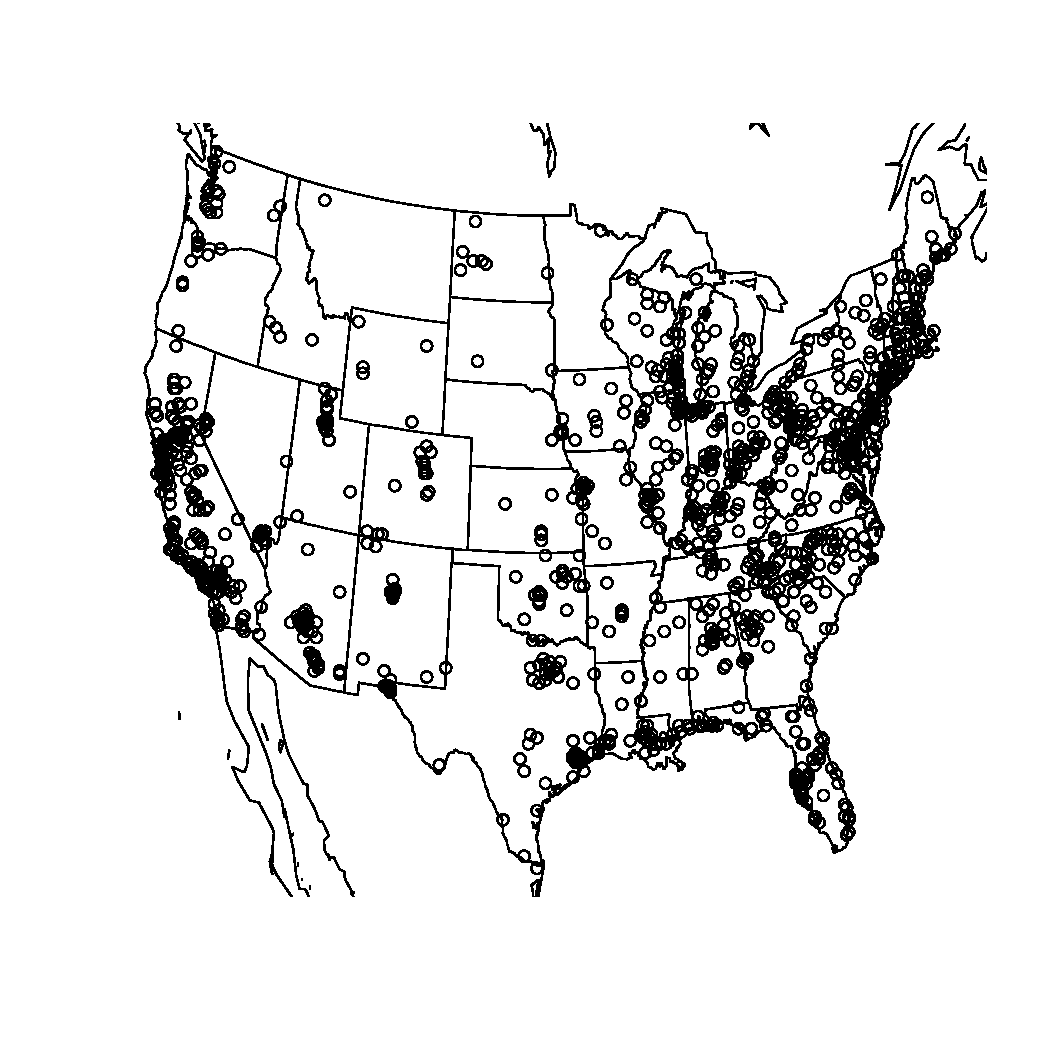
\includegraphics[width=1\linewidth]{./plots/pot/ozone_stations.pdf}
    \caption{Ozone monitoring station locations}
    \end{figure}
\end{columns}
\end{frame}

\begin{frame}{Data analysis}
  \centering
  \begin{figure}
    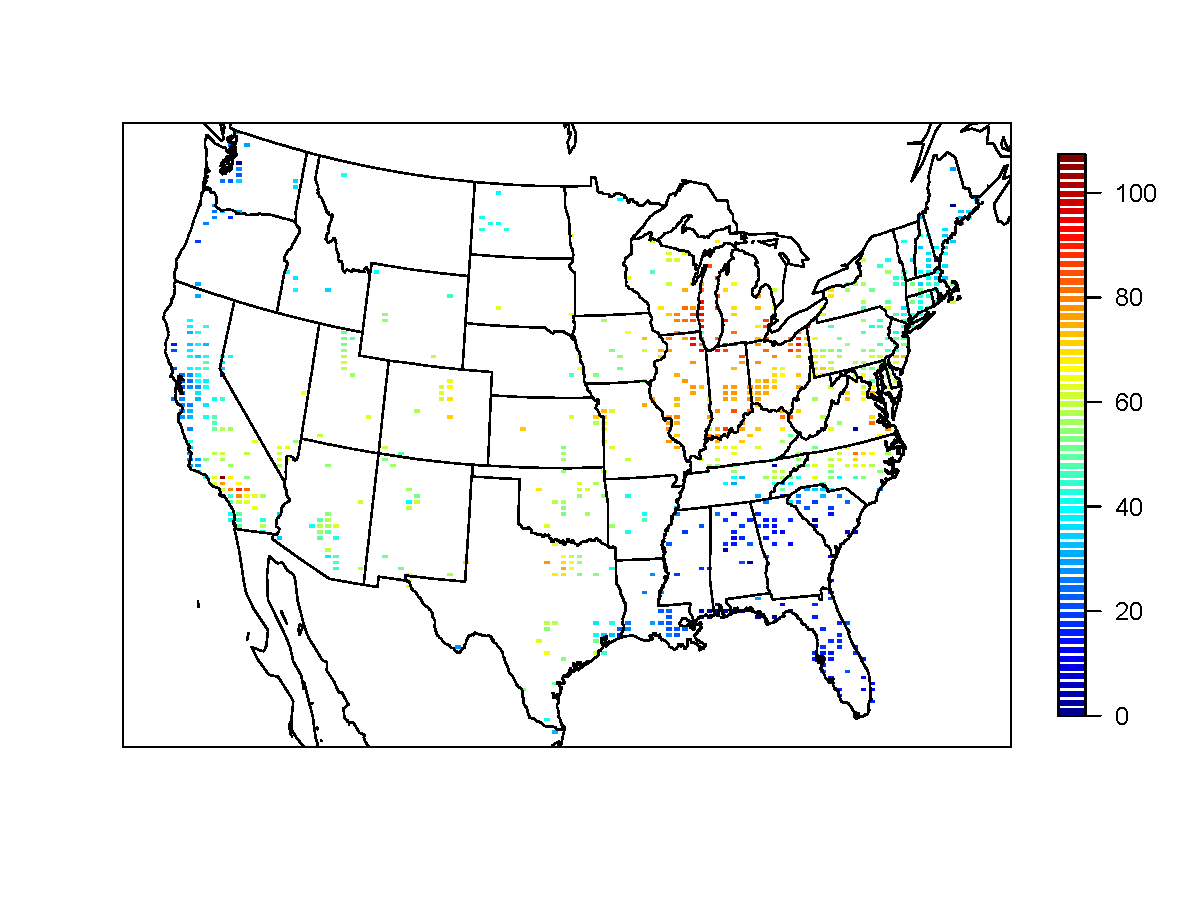
\includegraphics[width=\linewidth, trim=0 1in 0 0.7in ]{./plots/pot/ozone-10jul-us.pdf}
    \caption{Max 8-hour ozone measurements on July 10, 2005}
   \end{figure}
\end{frame}

% \begin{frame}{Exploratory data analysis}
% 	\centering
%   \begin{figure}
%     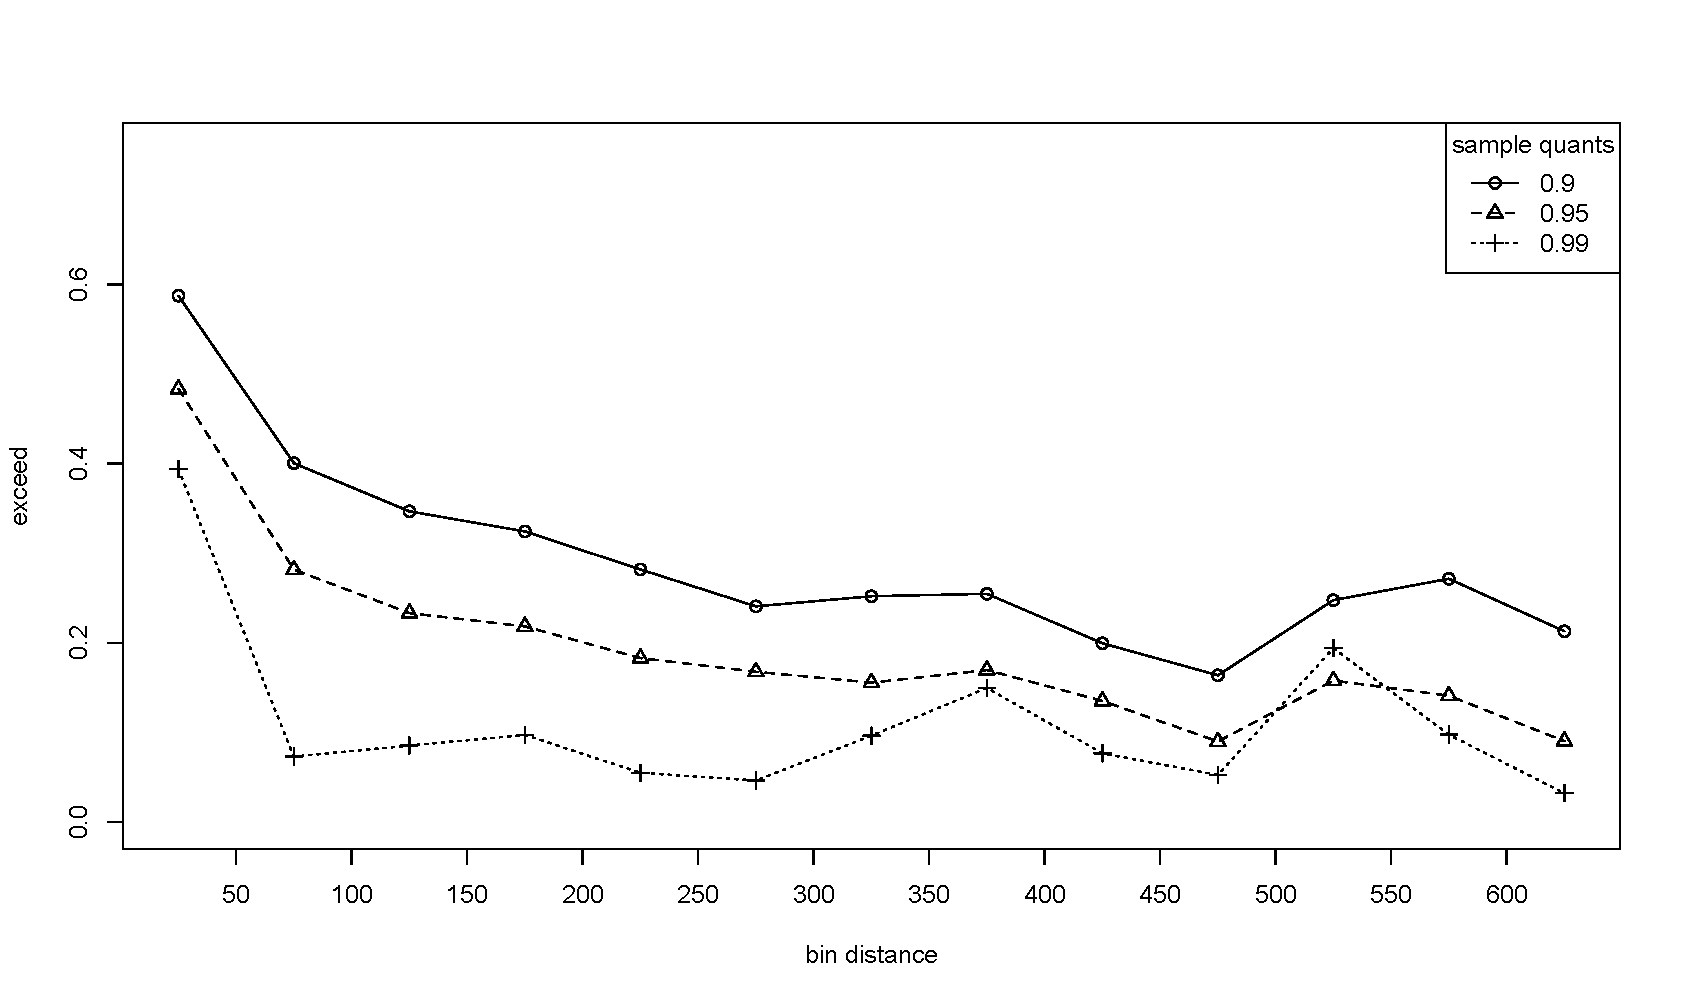
\includegraphics[width=1\linewidth, trim=0 0 0 1in]{./plots/pot/chi-plot-ozone-res.pdf}
%     \caption{$\widehat{\chi}$-plot for sample quantiles of ozone observations}
%   \end{figure}
% \end{frame}

\begin{frame}{Model comparisons}
  \begin{itemize} \setlength{\itemsep}{1em}
    \item 9 different analysis methods incorporating
    \begin{itemize}
      \item Gaussian vs $t$ vs skew-$t$ marginal distribution
      \item $K=1, 5, 6, 7, 8, 9, 10, 15$ partitions
      \item 4 threshold levels
      \begin{itemize}
         \item $T = 0$
         \item $T = 50$ppb, $q(0.48)$
         \item $T = 75$ppb, $q(0.92)$
         \item $T = 85$ppb, $q(0.97)$
      \end{itemize}
    \end{itemize}
    \item Compare Brier scores using two-fold cross validation
  \end{itemize}
\end{frame}

\begin{frame}{Model comparisons}
  \begin{itemize} \setlength{\itemsep}{1em}
    \item The Community Multiscale Air Quality (CMAQ) system provides fine-resolution simulated values for multiple air pollutants
    \item We use the tropospheric ozone output from the corresponding days in the CMAQ model as a covariate
    \item Mean function modeled as
    \begin{align*}
    	\bX_t(\bs) \bbeta = \beta_0 + \beta_1 \cdot \text{CMAQ}_t (\bs)
    \end{align*}
    \item All methods use a \Matern covariance
   \end{itemize}
\end{frame}

\begin{frame}{Cross-validation results}
  \centering
  \begin{figure}
    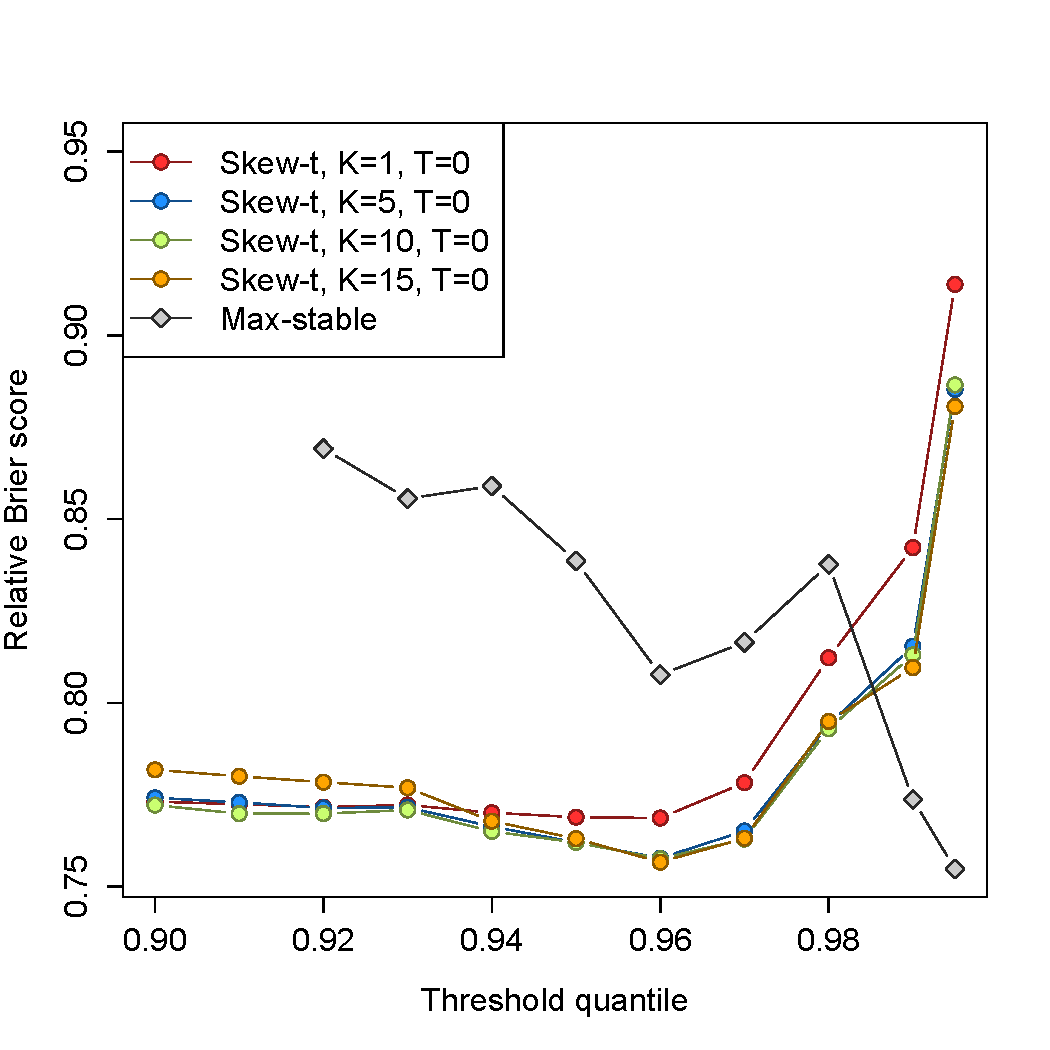
\includegraphics[width=0.6\linewidth, trim=0 0 0 1in]{./plots/pot/bs-ozone-1.pdf}
    % 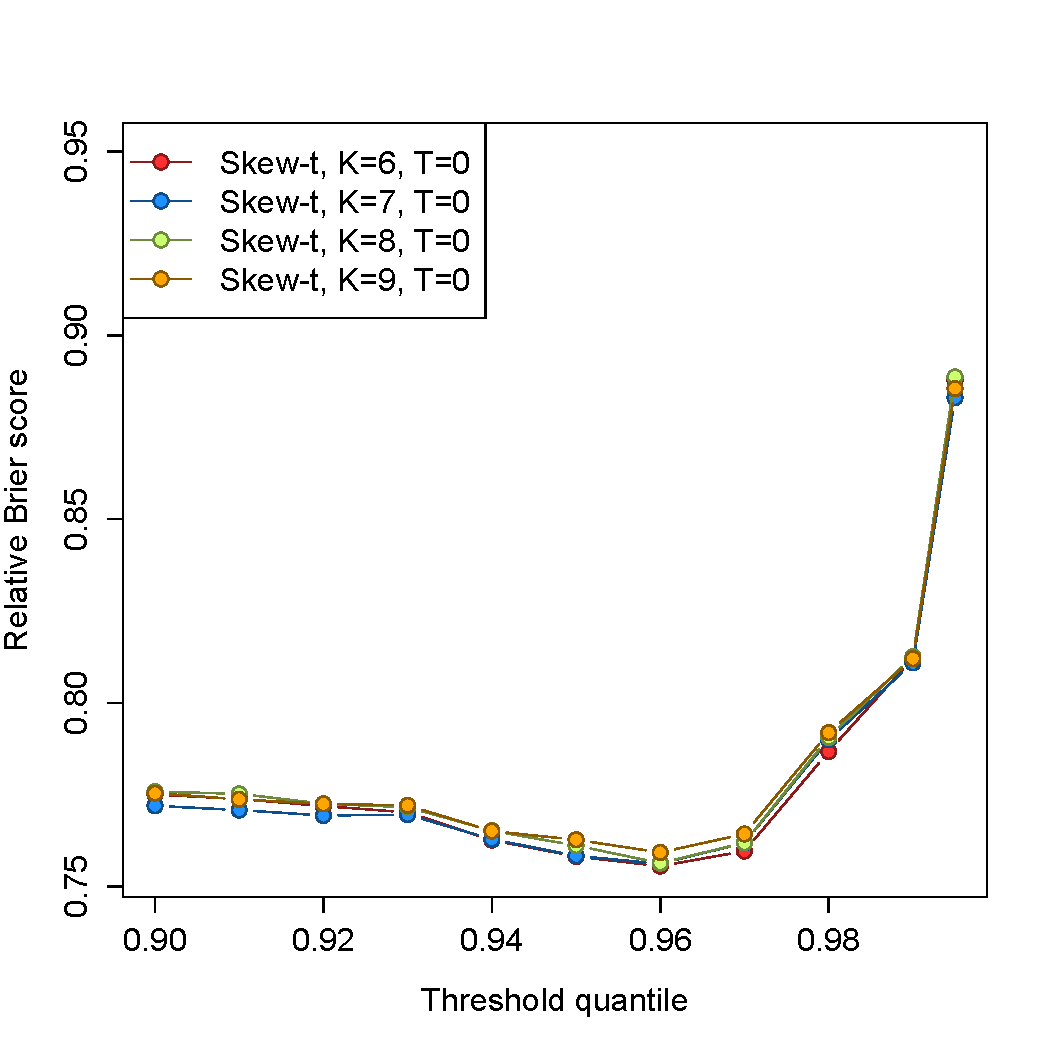
\includegraphics[width=0.47\linewidth]{./plots/pot/bs-ozone-2.pdf} \\
    \caption{Relative Brier score results ($K = 6$ -- $9$ are similar to $K = 5$ and $K = 10$)}
  \end{figure}
\end{frame}

\begin{frame}{Cross-validation results}
  \begin{itemize} \setlength{\itemsep}{1em}
    \item Key findings
    \begin{itemize}
      \item Partitioning improves performance across all high thresholds
      \item Models with anywhere from $K = 5$ to $K = 10$ partitions perform similarly
      \item In all cases, non-thresholded models perform better than thresholded models
    \end{itemize}
  \end{itemize}
\end{frame}

% % TODO: Update with new plots
% \begin{frame}{Predicted 95th quantile}
% \centering
% \begin{figure}
%     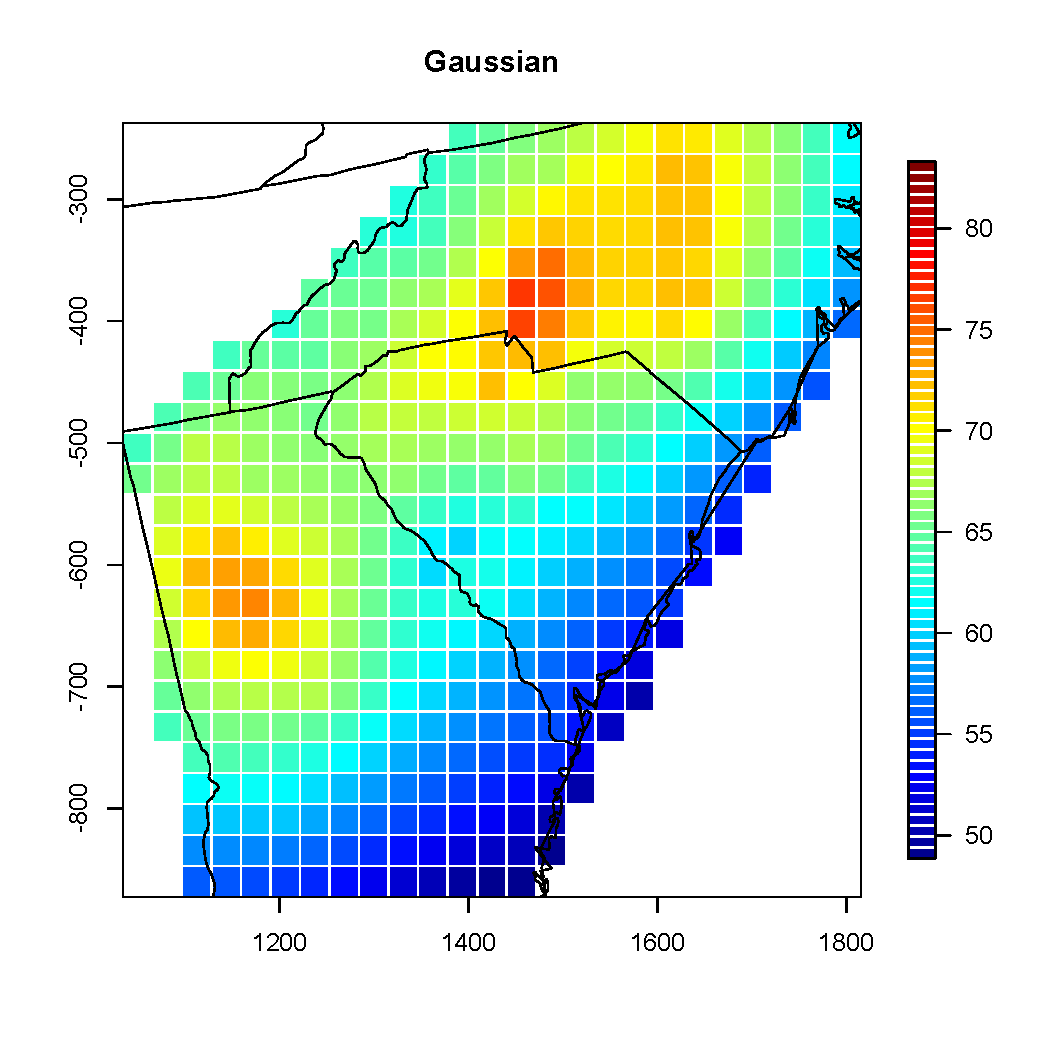
\includegraphics[width=.5\linewidth]{./plots/quantile-95-gau.pdf}
%     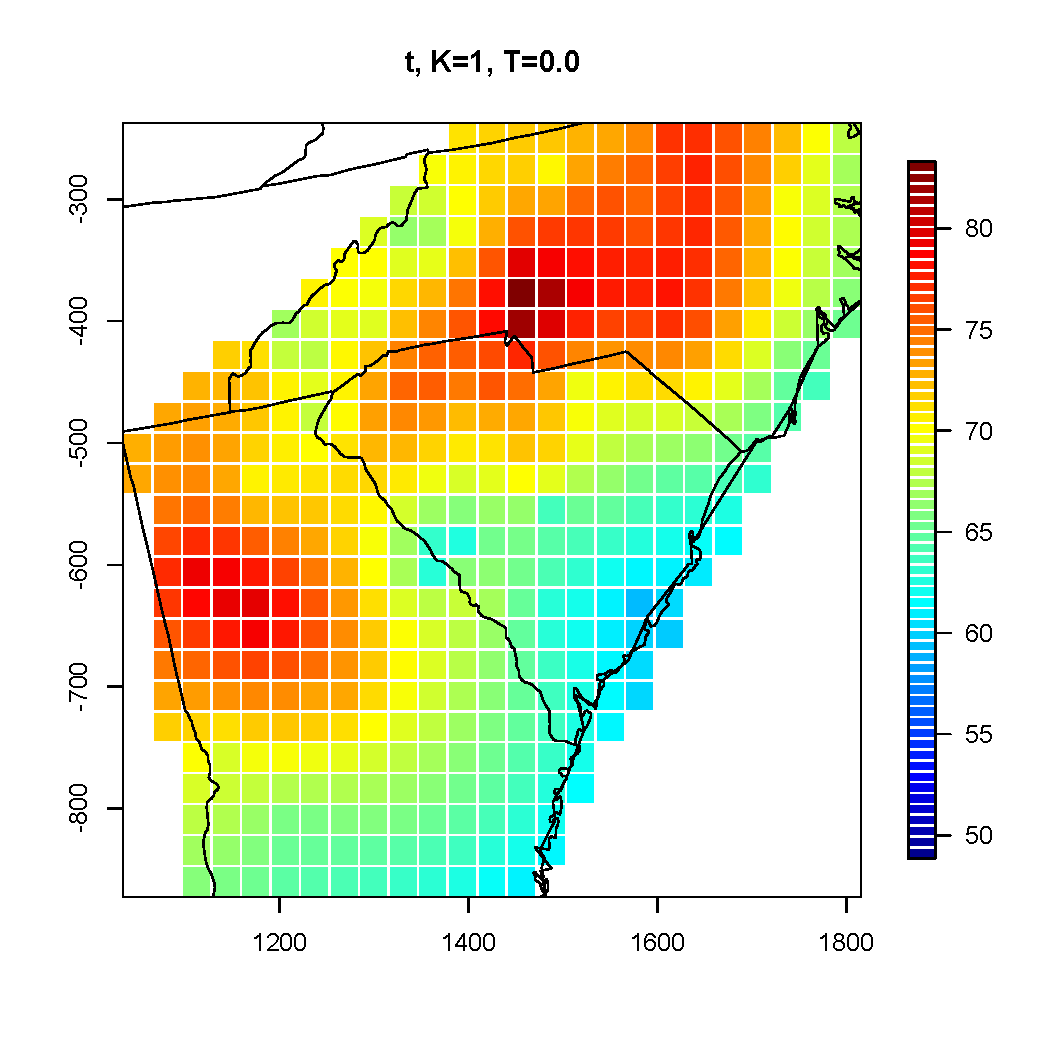
\includegraphics[width=.5\linewidth]{./plots/quantile-95-t10.pdf}
%     \caption{Predicted 95th quantile using Gaussian and $t$}
% \end{figure}
% \end{frame}

% \begin{frame}{Predicted 95th quantile}
% \centering
% \begin{figure}
%     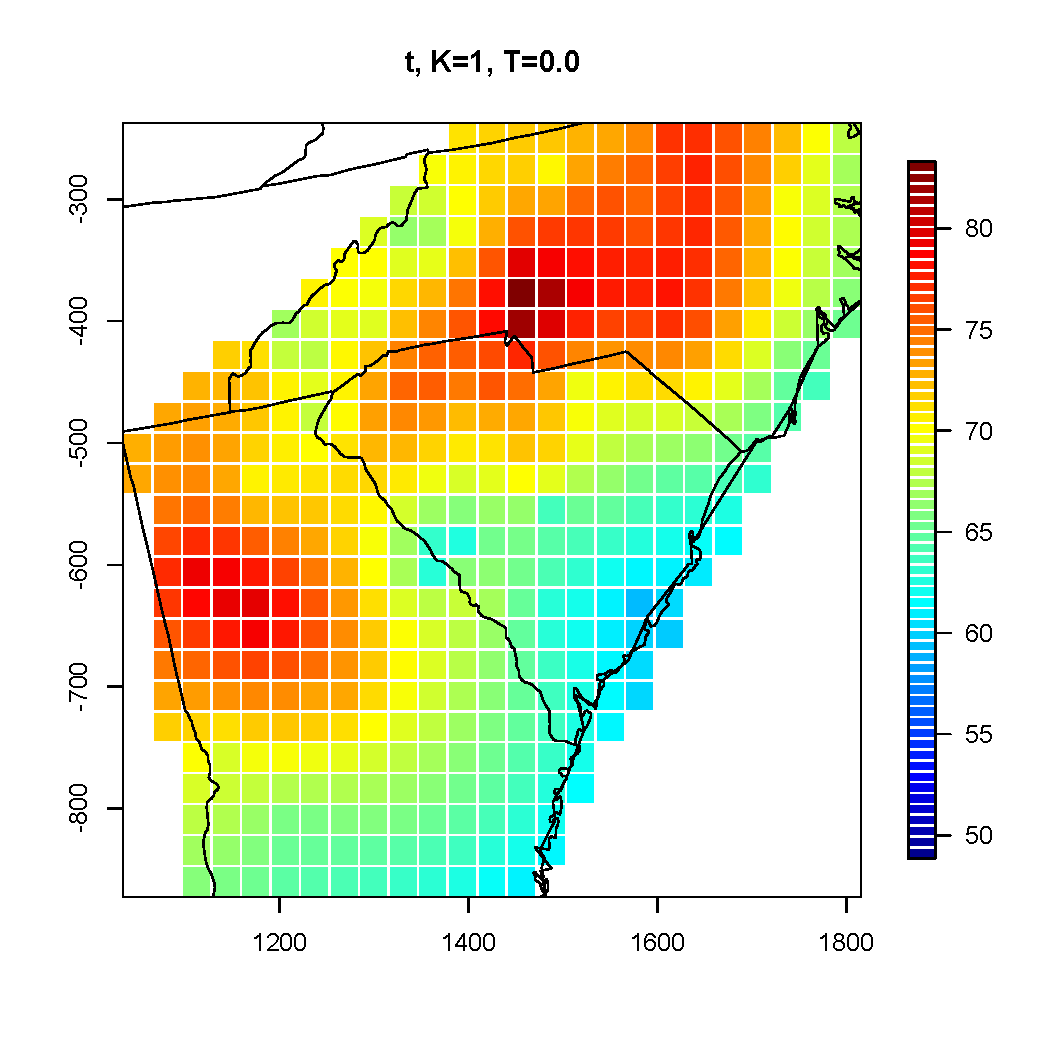
\includegraphics[width=.5\linewidth]{./plots/quantile-95-t10.pdf}
%     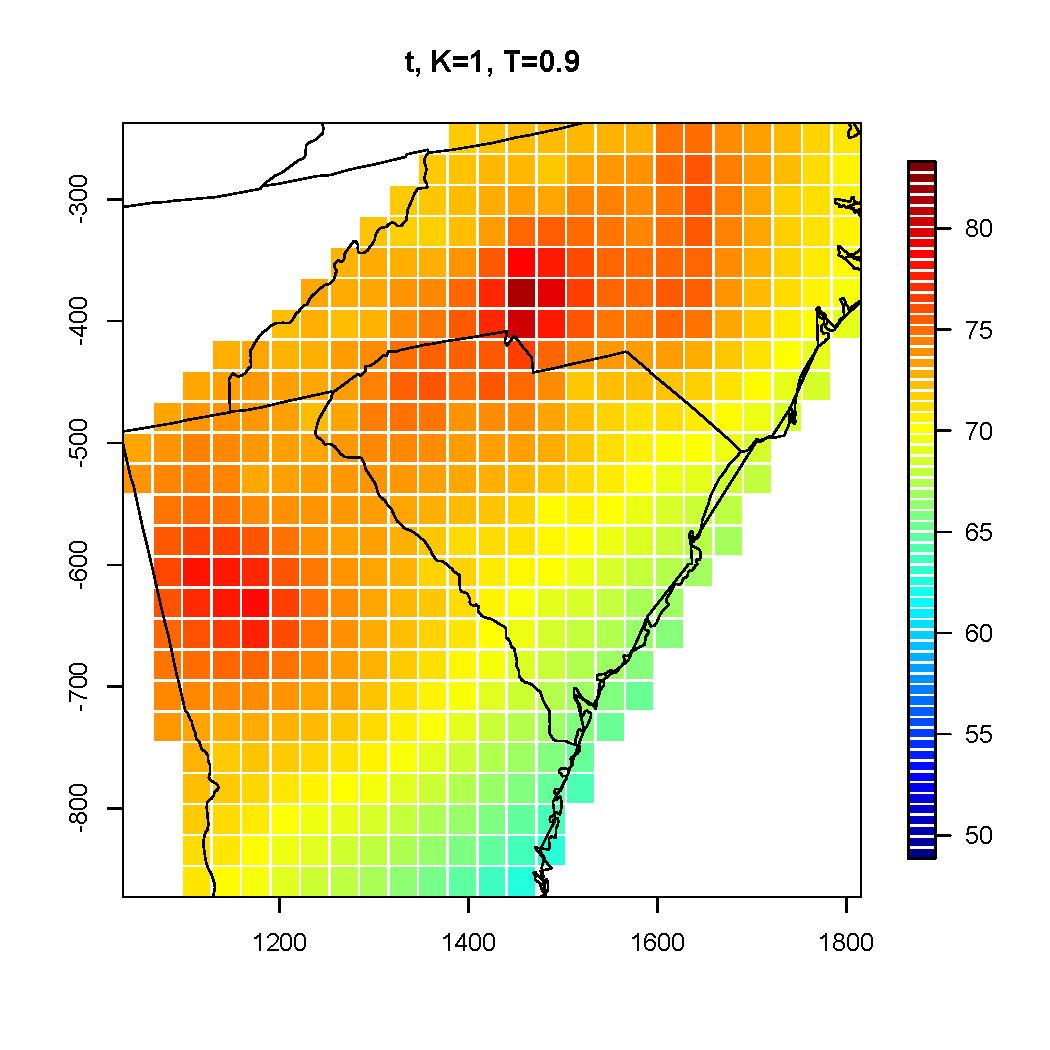
\includegraphics[width=.5\linewidth]{./plots/quantile-95-t19.pdf}
%     \caption{Predicted 95th quantile using $t$ and $t$ thresholded at $T=0.9$}
% \end{figure}
% \end{frame}

% \begin{frame}{Predicted 99th quantile}
% \centering
% \begin{figure}
%     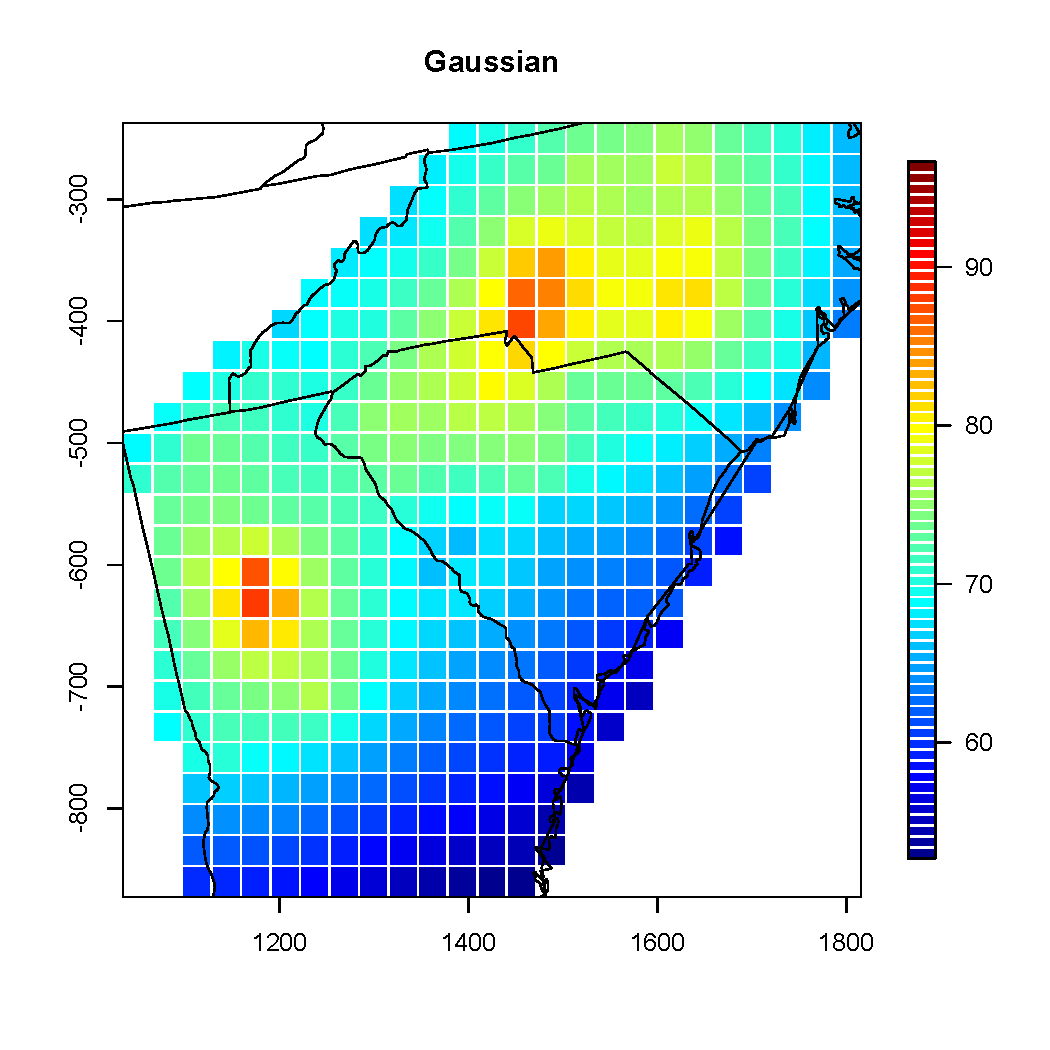
\includegraphics[width=.5\linewidth]{./plots/quantile-99-gau.pdf}
%     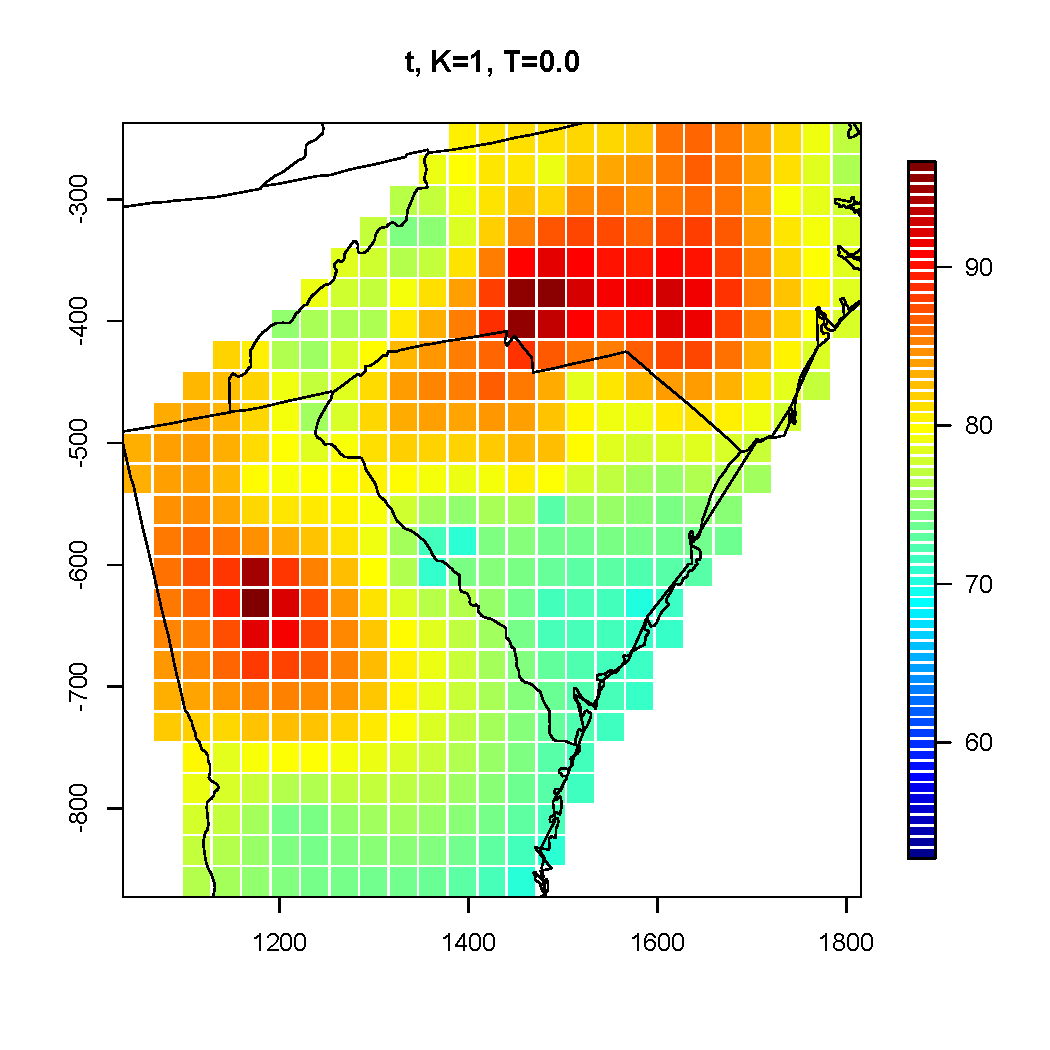
\includegraphics[width=.5\linewidth]{./plots/quantile-99-t10.pdf}
%     \caption{Predicted 99th quantile using Gaussian and $t$}
% \end{figure}
% \end{frame}

% \begin{frame}{Predicted 99th quantile}
% \centering
% \begin{figure}
%     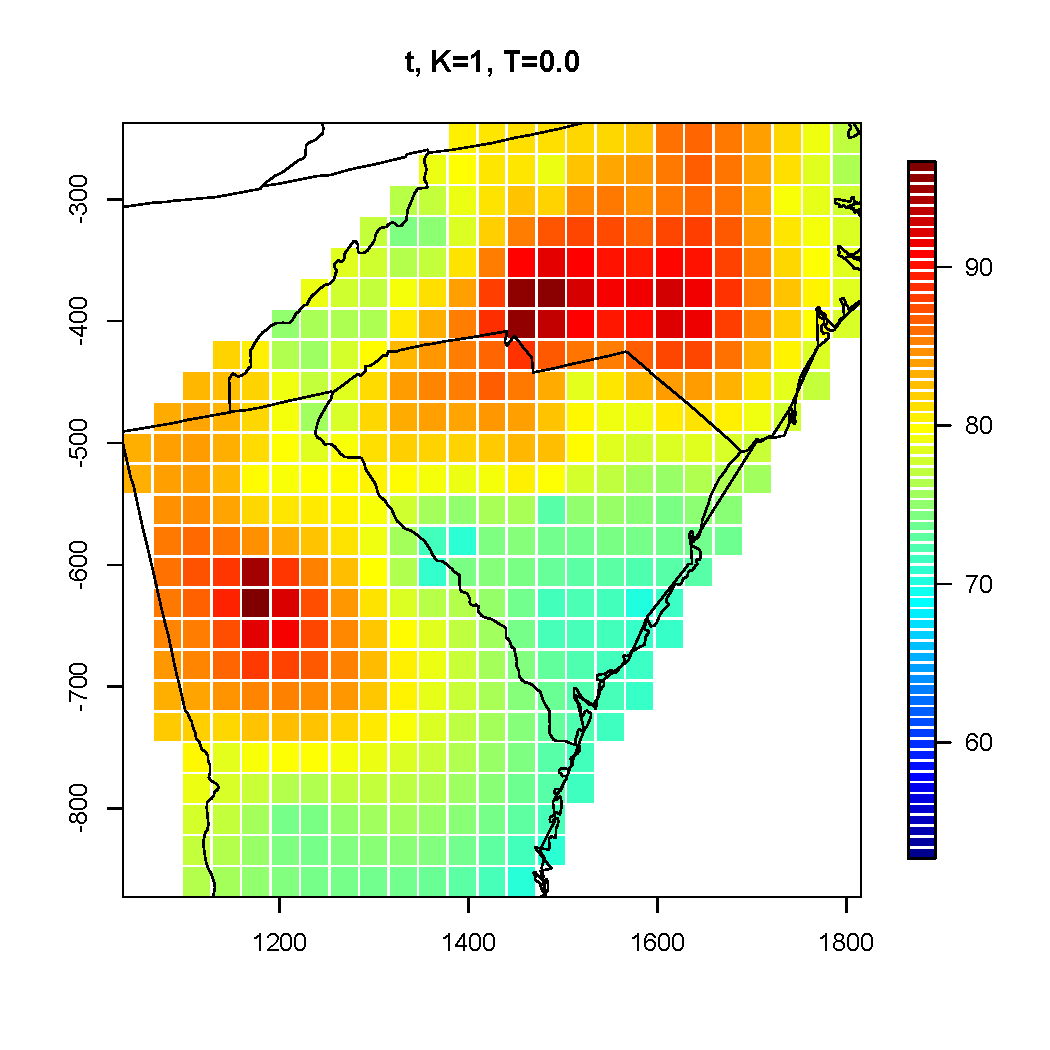
\includegraphics[width=.5\linewidth]{./plots/quantile-99-t10.pdf}
%     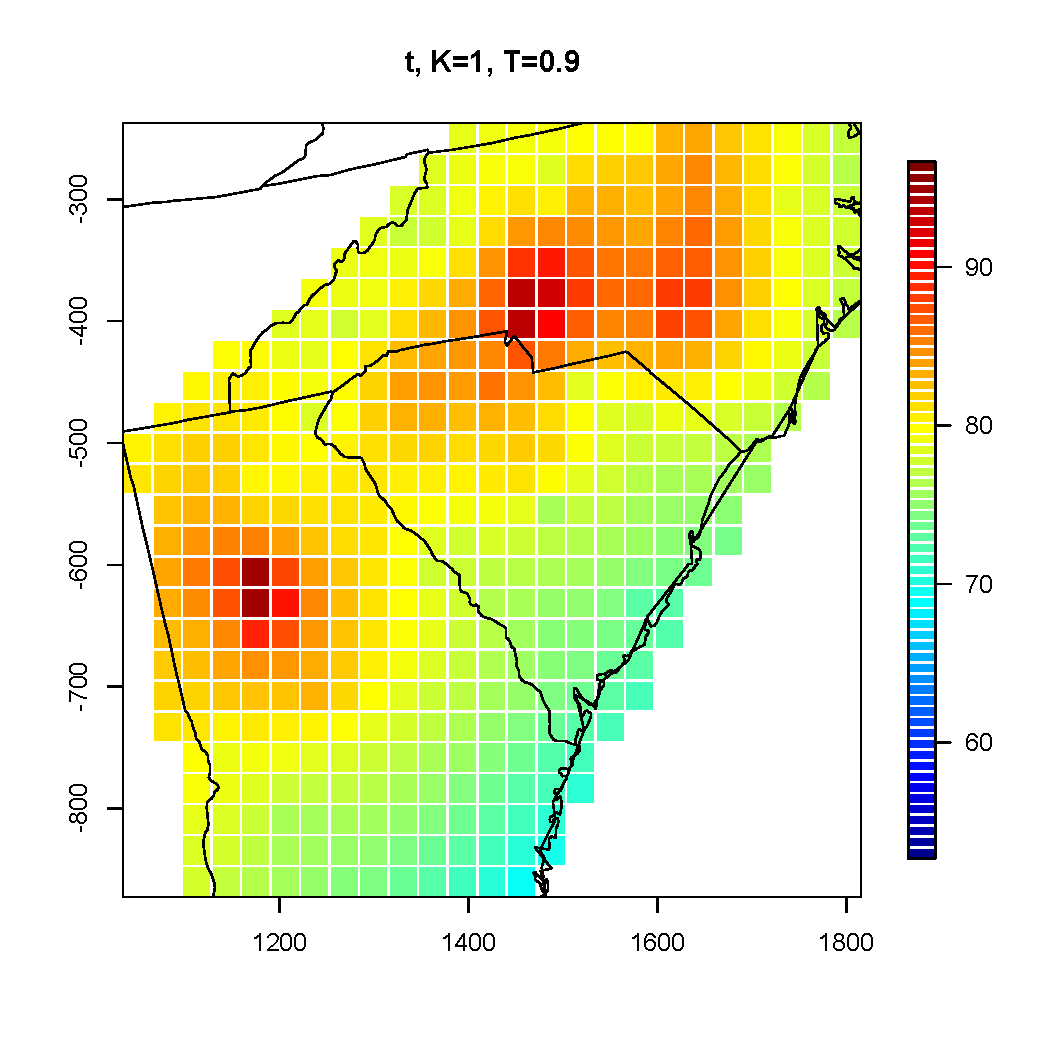
\includegraphics[width=.5\linewidth]{./plots/quantile-99-t19.pdf}
%     \caption{Predicted 99th quantile using $t$ and $t$ thresholded at $T=0.9$}
% \end{figure}
% \end{frame}

% \begin{frame}{Probability of exceedance}
% \centering
% \begin{figure}
%     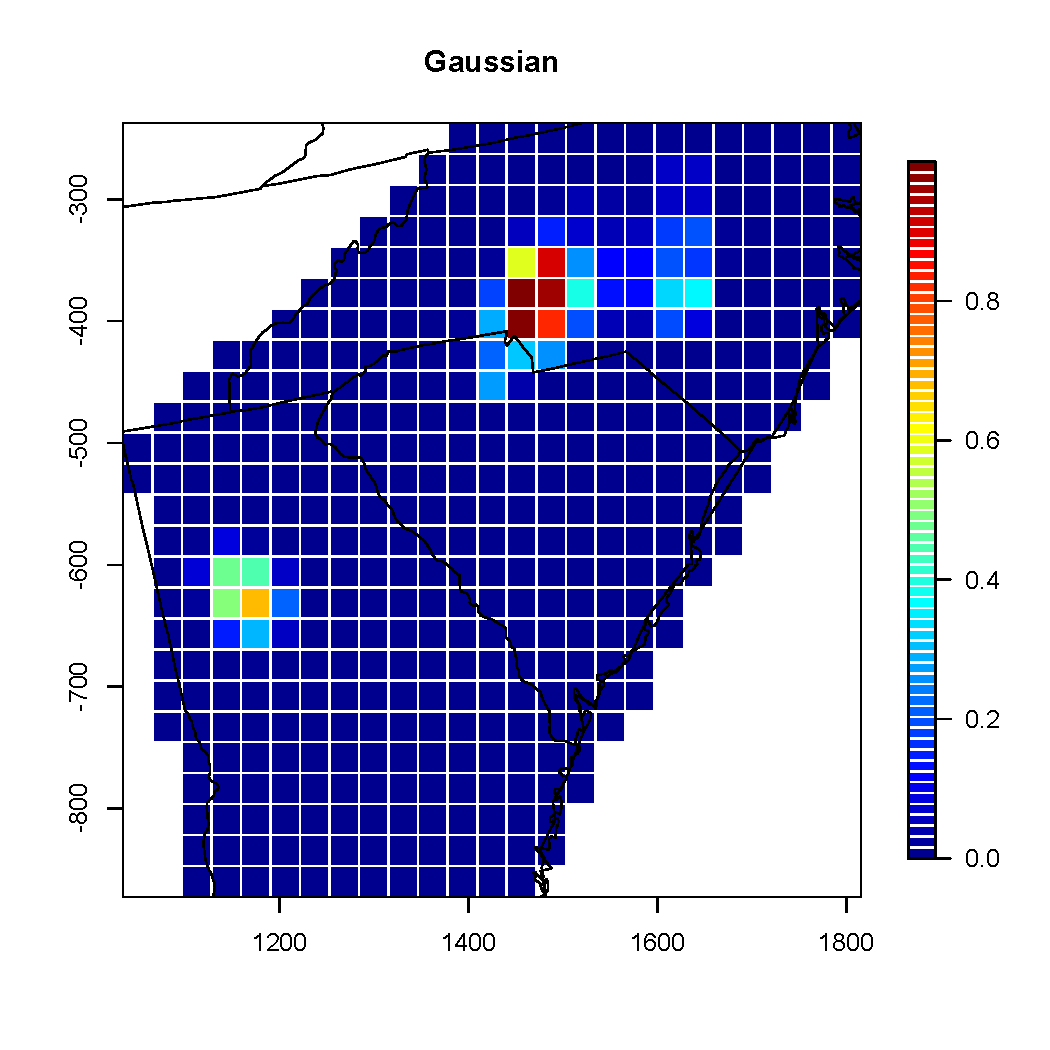
\includegraphics[width=.5\linewidth]{./plots/p-exceed-std-gau.pdf}
%     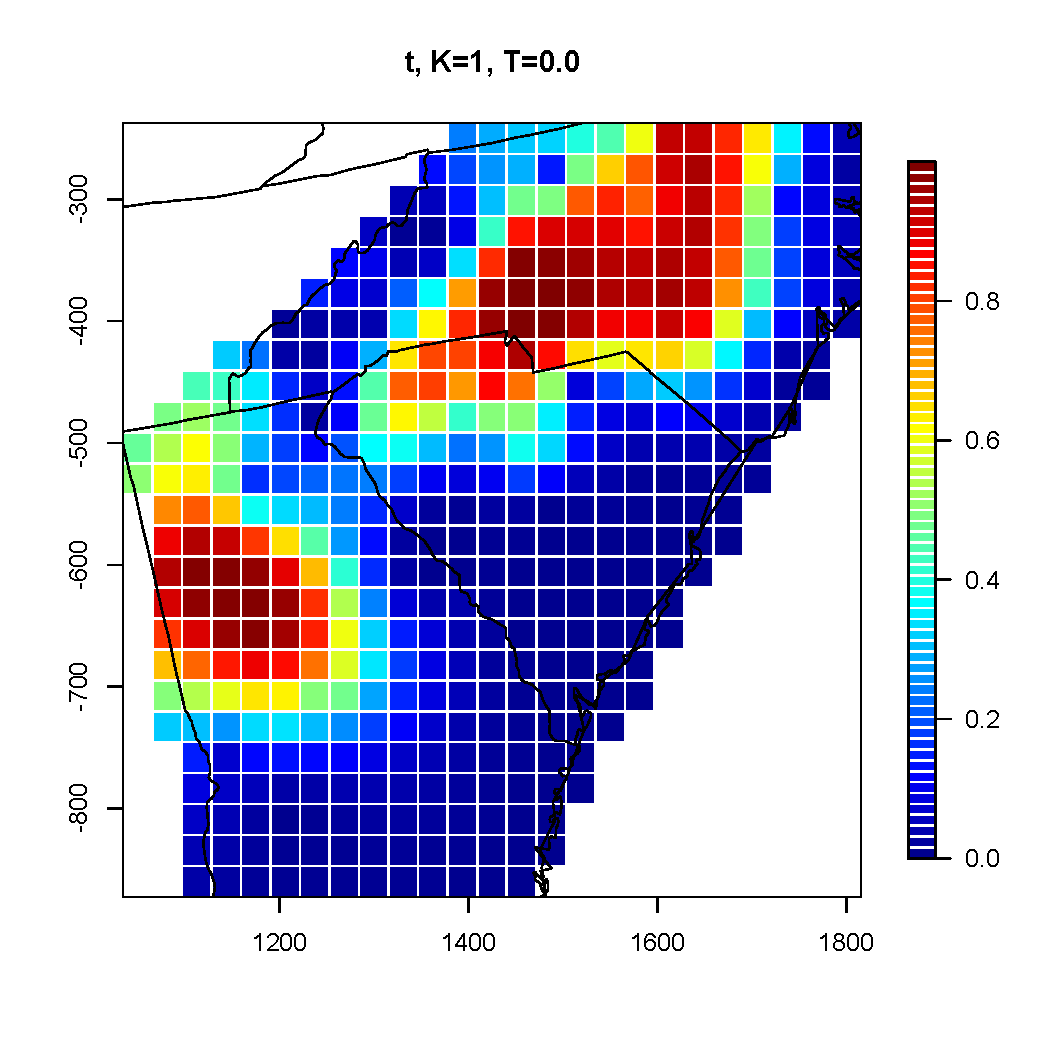
\includegraphics[width=.5\linewidth]{./plots/p-exceed-std-t10.pdf}
%     \caption{Probability of exceeding the 75 ppb ozone standard using Gaussian and $t$}
% \end{figure}
% \end{frame}

% \begin{frame}{Probability of exceedance}
% \centering
% \begin{figure}
%     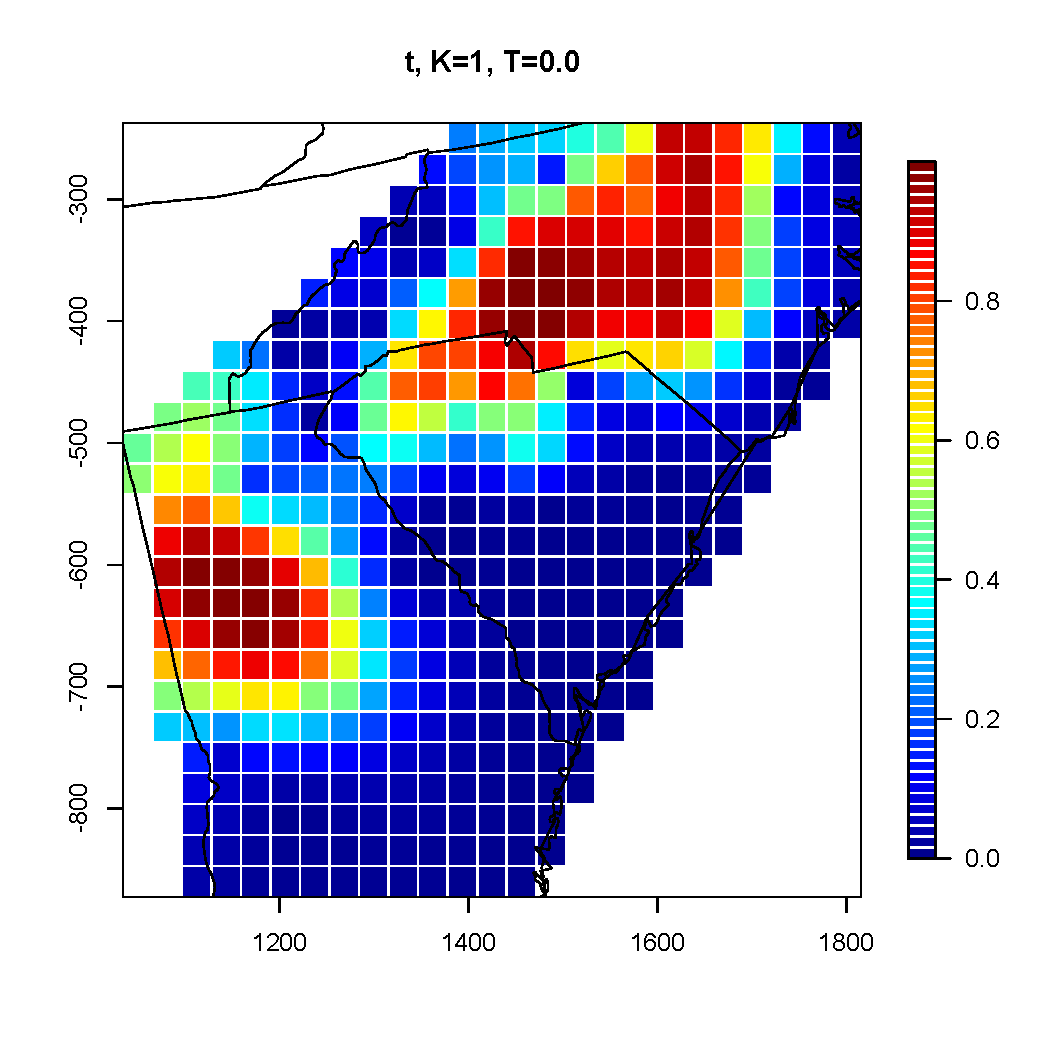
\includegraphics[width=.5\linewidth]{./plots/p-exceed-std-t10.pdf}
%     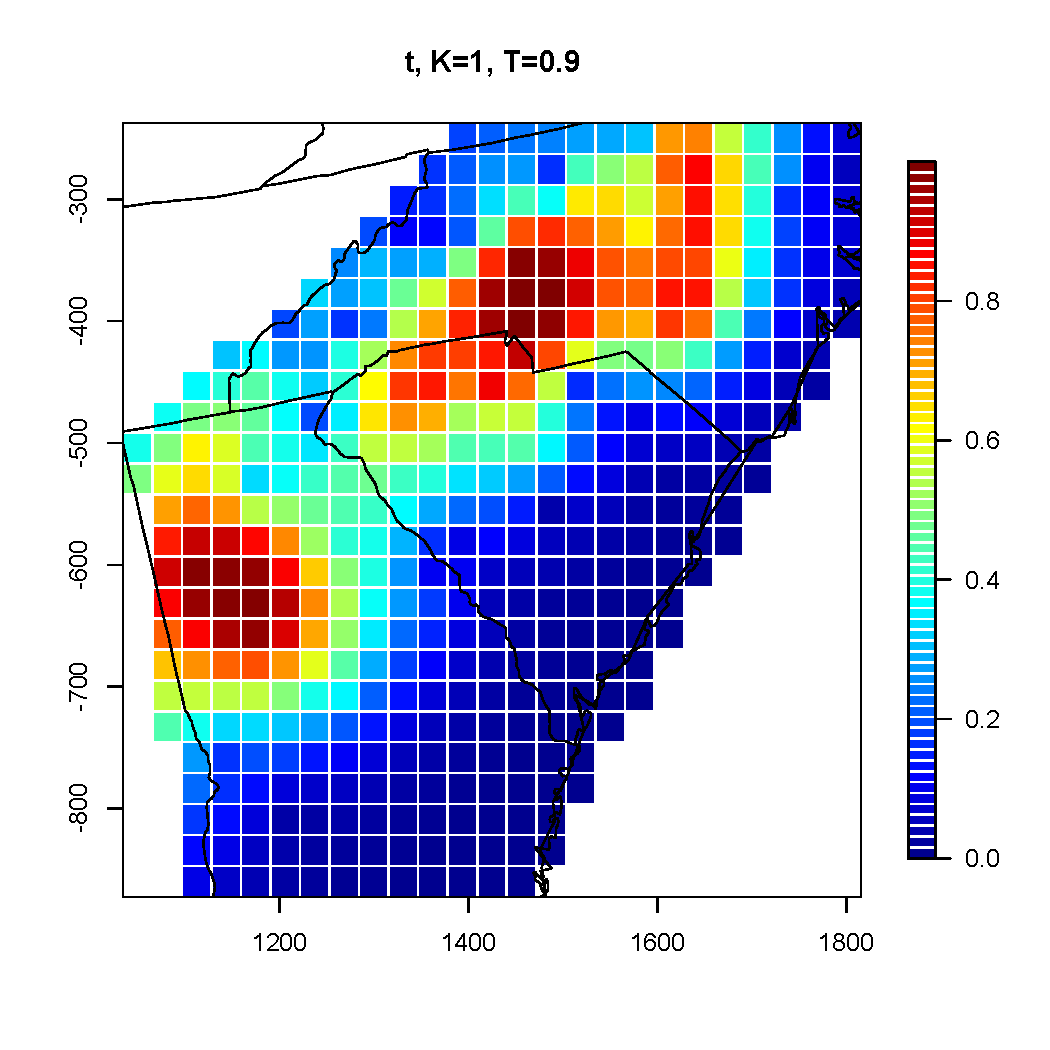
\includegraphics[width=.5\linewidth]{./plots/p-exceed-std-t19.pdf}
%     \caption{Probability of exceeding the 75 ppb ozone standard using $t$ and $t$ thresholded at $T=0.9$}
% \end{figure}
% \end{frame}

\begin{frame}{Discussion}
  \begin{itemize} \setlength{\itemsep}{1em}
    \item Improvement of model performance when using partitioned models
    \item Thresholding makes results worse
    \begin{itemize}
      \item Possible numerical instability due to truncated normal distribution
    \end{itemize}
  \end{itemize}
\end{frame}

\begin{frame}{Future work: Knots and their impact}
  \begin{itemize} \setlength{\itemsep}{1em}
    \item Different partition structure
    \begin{itemize}
      \item Distance weighting for each knot vs indicator functions
    \end{itemize}
    \item Knot selection
    \begin{itemize}
      \item Possible prior on the probability a knot is in the spatial domain
    \end{itemize}
  \end{itemize}
\end{frame}

\begin{frame}{Future work: Temporal dependence}
  \begin{itemize} \setlength{\itemsep}{1em}
    \item Temporal dependence should be accounted for when using daily data
    \item For multiple days of observations the model becomes
      \begin{align*}
        Y_t(\bs) = \bX_t(\bs)^T \bbeta + \lambda \sigma_t(\bs) | z_t(\bs) | + \sigma_t(\bs) v_t(\bs)
      \end{align*}
      where $t$ denotes the day of each observation
    \item Different ways to incorporate the temporal dependence
    \begin{itemize}
      \item Time series on $\bw_t$, $z_t(\bs)$, and $\sigma_t(\bs)$
      \item Three dimensional covariance model for $v_t(\bs)$ (e.g. Huser and Davison, 2014)
    \end{itemize}
  \end{itemize}
\end{frame}

\begin{frame}{Future work: Temporal dependence}
  \begin{itemize} \setlength{\itemsep}{1em}
    \item We choose the time series approach because the $z_t(\bs)$ and $\sigma_t(\bs)$ terms dictate the tail behavior
    \item We incorporate an AR(1) time series on $\bw^*_{tk} = (w^*_{tk1}, w^*_{tk2})$, $z_{tk}$, and $\sigma^*_{tk}$ where
    \begin{align*}
      w^*_{tki} &= \Phi^{-1}\left[ \frac{w_{tki} - \min(\bs_i)}{ \text{range}(\bs_i)}\right] \quad i = 1, 2 \\[0.5em]
      \sigma^{2*}_t(\bs) &= \Phi^{-1}\{ \text{IG}[\sigma^2_t(\bs)] \}
    \end{align*}
    are transformations to $\calR^2$
  \end{itemize}
\end{frame}

\begin{frame}{Rare binary regression}
  \begin{itemize} \setlength{\itemsep}{1em}
    \item Motivation
    \begin{itemize}
      \item Want to incorporate spatial dependence when modeling rare events (e.g. Diseased trees, Disease outbreak, Crimes)
    \end{itemize}
    \item We observe
    \begin{align*}
      Y_i = \left\{ \begin{array}{ll}
        1 \quad & \text{event occurred}\\
        0 \quad & \text{no event occurred}
      \end{array} \right.
    \end{align*}
    \item We model $\Pr[Y_i = 1]$
  \end{itemize}
\end{frame}

\begin{frame}{Rare binary regression}
  \begin{itemize} \setlength{\itemsep}{1em}
    \item Common examples with non-spatial analysis
    \begin{itemize}
      \item Logistic regression
      \begin{align*}
        \Pr[Y_i = 1] = \frac{ \exp(\bX_i \bbeta) }{ 1 + \exp(\bX_i \bbeta)}
      \end{align*}
      \item Probit regression
      \begin{align*}
        \Pr[Y_i = 1] = \Phi(\bX_i \bbeta)
      \end{align*}
      where $\Phi$ is the standard normal distribution function
      \item Cloglog regression
      \begin{align*}
        \Pr[Y_i = 1] = 1 - \exp[ -\exp(\bX_i \bbeta)]
      \end{align*}
    \end{itemize}
  \end{itemize}
\end{frame}

\begin{frame}{Rare binary regression}
  \begin{itemize} \setlength{\itemsep}{1em}
    \item Generalized extreme value link function (Wang and Dey, 2010)
    \begin{align*}
      \Pr[Y_i = 1] = 1 - \exp\left[-(1 - \xi \bX_i \bbeta)^{-1 / \xi} \right]
    \end{align*}
    \item Link function allows for greater positive skew than existing methods
    \begin{itemize}
      \item When $\xi = 0$, the link is the Cloglog link
      \item When $\xi > 0$, the link allows for greater positive skew than Cloglog link
    \end{itemize}
  \end{itemize}
\end{frame}

\begin{frame}{Rare spatial binary regression}
  \begin{itemize} \setlength{\itemsep}{1em}
    \item We propose to develop a spatial model
    \item Objectives are to borrow strength across sites to estimate covariate effects and spatial prediction
    \item Proposed method will
    \begin{itemize}
      \item Use the GEV link function
      \item Use the hierarchical method for spatially dependent extremes from Reich and Shaby (2012)
    \end{itemize}
    \item Model parameters fit using MCMC
  \end{itemize}
\end{frame}

\begin{frame}{Rare spatial binary regression}
  \begin{itemize} \setlength{\itemsep}{1em}
    \item We model $Y_i = I(Z_i > 0)$ where $z_i\sim$ multivariate GEV (mGEV)  is a latent variable
    \item Hierarchical model for mGEV (Reich and Shaby, 2012)
    \begin{itemize}
      \item $Z(\bs) = U(\bs) \theta(\bs)$
      \begin{itemize}
        \item $U(\bs) \iid$ GEV(1, $\alpha$, $\alpha$) is a nugget effect
        \item $\theta(\bs) = [\sum_{l = 1}^L A_l w_l(\bs)^{1/\alpha}]^\alpha$ is the spatial process
        \item $\alpha \in (0, 1)$ controls strength of nugget relative to spatial dependence
        \item $A_l \iid$ Positive Stable($\alpha$) is an random effect representing the intensity
        \item $w_l(\bs)$ gives the weight of the intensity of the $l$th random effect on site $\bs$
      \end{itemize}
    \end{itemize}
  \end{itemize}
\end{frame}

\begin{frame}{Likelihood function}
  \begin{itemize} \setlength{\itemsep}{1em}
    \item After marginalizing out the $A_l$ terms, we have the asymmetric logistic dependence function (Reich and Shaby, 2012)
    \footnotesize{
    \begin{align*}
      G(\bz) = \Pr[Z_1 < z_z, \ldots, Z_n < z_n] = \exp\left\{ - \sum_{l = 1}^{L} \left[ \sum_{i = 1}^n \left( \frac{ w_l(\bs_i) }{ z_i } \right)^{ 1 / \alpha} \right]^\alpha \right\}
    \end{align*}
    }
    where
    \begin{itemize}
      \item $w_l$ is a weighting function subject to the constraint that $\sum_{l = 1}^L w_l = 1$
      \item $\alpha$ controls spatial dependence
      \begin{itemize}
        \item $\alpha = 0$ is strong dependence
        \item $\alpha = 1$ is joint independence
      \end{itemize}
    \end{itemize}
  \end{itemize}
\end{frame}

\begin{frame}{Weighting function}
  \begin{itemize} \setlength{\itemsep}{1em}
    \item We use the Gaussian weights proposed by Reich and Shaby (2012) given by
    \footnotesize{
    \begin{align*}
      w_l(\bs_i) = \frac{ \exp\left[ -0.5 \left( \frac{ || \bs_i - \bv_l || }{ \rho} \right)^2 \right]}{ \sum_{l = 1}^L \exp\left[ -0.5 \left( \frac{ || \bs_i - \bv_l || }{ \rho} \right)^2 \right] }
    \end{align*}
    }
    where
    \begin{itemize}
      \item $\bv_l$ are spatial knots
      \item $\rho$ is a bandwidth term for the kernel function
    \end{itemize}
  \end{itemize}
\end{frame}

\begin{frame}{Illustrating asymmetric logistic dependence in one-dimension}
  \centering
  \begin{figure}
    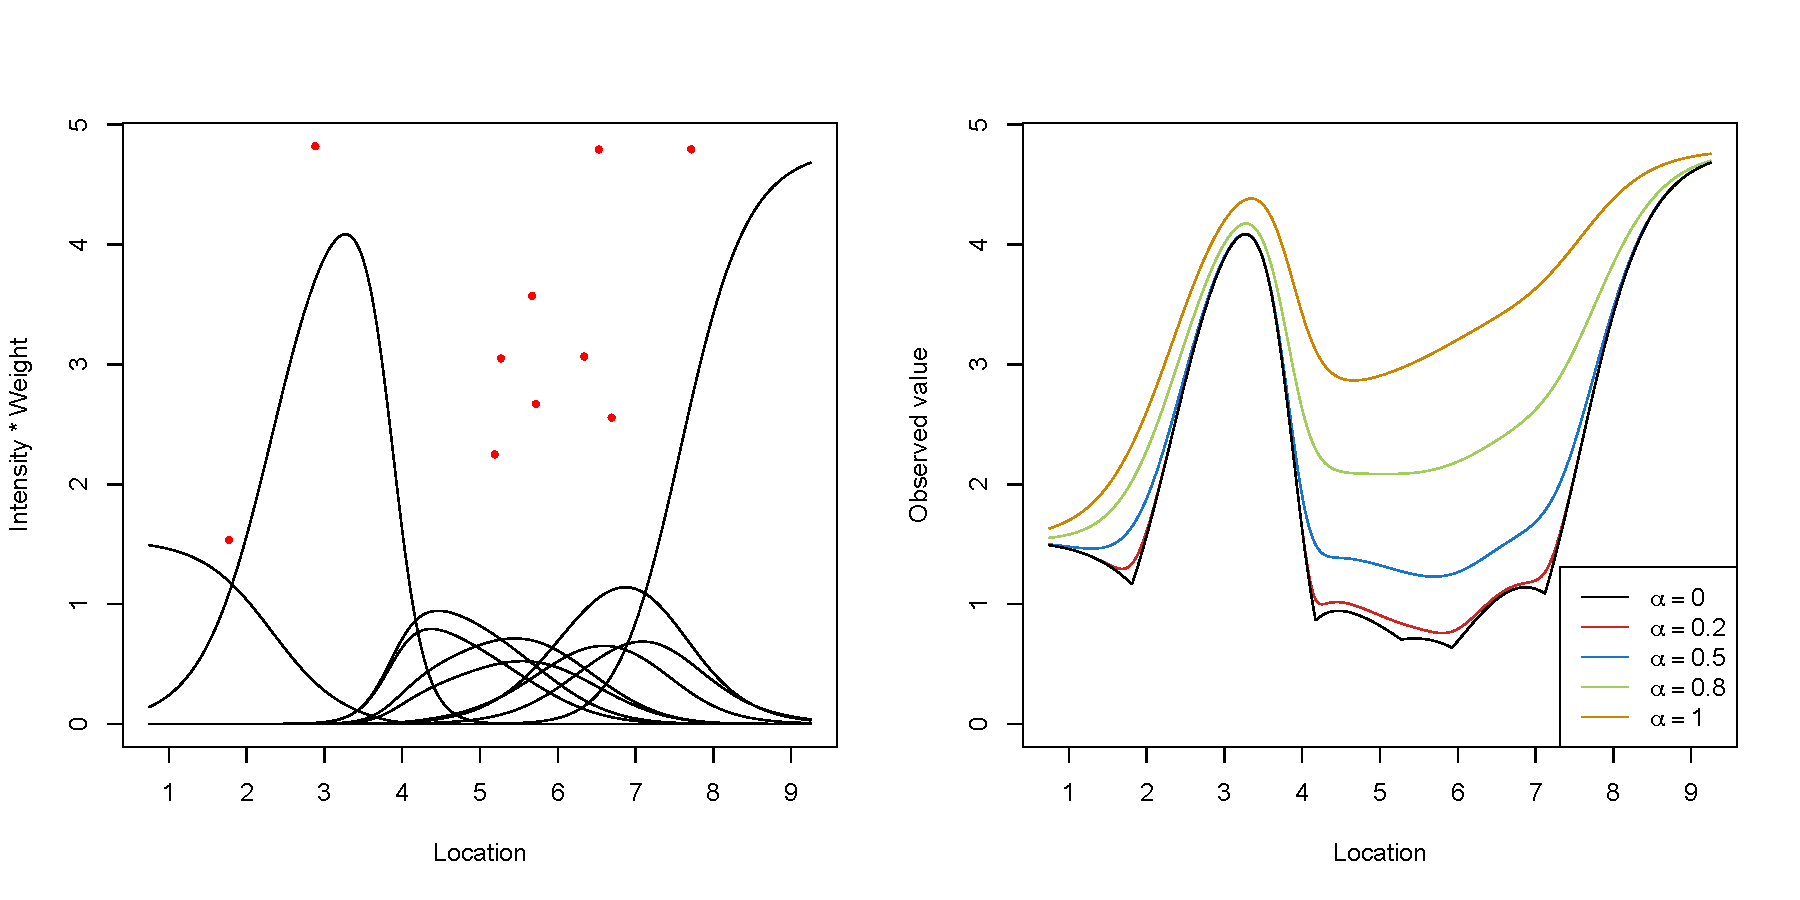
\includegraphics[width=\linewidth, trim=0 0.5in 0 0]{./plots/max-stable.pdf}
    \caption{Knot intensity $\times$ weight ($\rho = 0.5$), red dots give intensity of random effects (left) Impact of $\alpha$ (right).}
   \end{figure}
\end{frame}

\begin{frame}{Joint likelihood}
  \begin{itemize} \setlength{\itemsep}{1em}
    \item Let $K_t = \sum_{i = 1}^n Y_{it}$ be the number of exceedances that occur on day $t$.
    \item Rearrange the sites so
    \begin{itemize}
      \item $Y_1, \ldots, Y_K$ are the observations where $Y(\bs_i) = 1$
      \item $Y_{K+1}, \ldots, Y_n$ are the observations where $Y(\bs_i) = 0$
    \end{itemize}
    \item Then for $K = 0, 1, 2$
    {\scriptsize
    \begin{align*}
      \Pr(Y_1 = y_1, \ldots, Y_n = y_n) = \left\{ \begin{array}{ll}
        G(\bz)  & K = 0\\
        G(\bz_{(1)}) - G(\bz) & K = 1\\
        G(\bz_{(12)}) - G(\bz_{(1)}) - G(\bz_{(2)}) + G(\bz) & K =2
      \end{array}\right.
    \end{align*}
    }
    where $G\left(\bz_{(1)}\right) = \Pr(Z_2 < z_2, \ldots, Z_n < z_n)$
    \item $K > 2$ can be derived similarly
  \end{itemize}
\end{frame}

\begin{frame}{Joint likelihood}
  \begin{itemize} \setlength{\itemsep}{1em}
    \item For small $K$, we can evaluate the likelihood directly
    \item For large $K$, we use the hierarchical model of Reich and Shaby (2012)
  \end{itemize}
\end{frame}

\begin{frame}{Future simulation study and data application}
  \begin{itemize} \setlength{\itemsep}{1em}
    \item Simulation study
    \begin{itemize}
      \item Data generated using logistic, Cloglog, and GEV links
      \begin{itemize}
        \item Exploring how rarity of event impacts prediction
      \end{itemize}
      \item Models fit using
      \begin{itemize}
        \item mGEV
        \item Random effects Gaussian distribution
      \end{itemize}
    \end{itemize}
    \item Data application: Modeling crime data
    \begin{itemize}
      \item Homicides, car theft, vandalism
    \end{itemize}
  \end{itemize}
\end{frame}


% TODO: more about this model for sure
\begin{frame}{Non-stationary covariance for extreme values}
  \begin{itemize} \setlength{\itemsep}{1em}
    \item Stationary covariance functions are a function of distance between two sites.
    \begin{align*}
      \rho[Y(\bs), Y(\bt)] = \rho(h)
    \end{align*}
    where $h = ||\bs - \bt||$
    \item This assumes the covariance is the same everywhere, e.g. east vs west, mountains vs desert
    \item Misspecifying the covariance can impair spatial prediction and statistical inference
  \end{itemize}
\end{frame}

\begin{frame}{Non-stationary covariance for extreme values}
  \begin{itemize} \setlength{\itemsep}{1em}
    \item In extremes, stationary extremal dependence means
    \begin{align*}
      \chi(h) = \Pr[Y(\bs) > c | Y(\bt) > c]
    \end{align*}
    \item Currently, there are no methods to model non-stationarity in spatial extremes
    \item Semiparamtric approach using spectral density ratios (de Carvalho and Davison, 2014)
    \begin{itemize}
      \item Vector of observations can be transformed to psuedo-polar coordinates
      \item Pairwise analysis
    \end{itemize}
    \item New approach extending Reich and Shaby (2012)
    \begin{itemize}
      \item Current model uses a single bandwidth term $\rho$ for all knots
      \item Proposed idea is to implement a knot-specific $\rho$ to induce non-stationarity
    \end{itemize}
  \end{itemize}
\end{frame}


\begin{frame}{Thesis outline}
  \begin{itemize} \setlength{\itemsep}{1em}
    \item Chapter 1: Review of extreme value theory \alert{August 2015}
    \item Chapter 2: Spatiotemporal model for extreme value analysis based on the skew-$t$ distribution \alert{February 2015}
    \item Chapter 3: Rare spatial binary regression \alert{May / June 2015}
    \item Chapter 4: Non-stationary covariance through knot-specific bandwidth \alert{August 2015}
  \end{itemize}
\end{frame}

\begin{frame}{Questions}
  \begin{itemize} \setlength{\itemsep}{1em}
    \item Questions?
    \item Thank you for your attention.
    \item Acknowledgment: This work was funded by EPA STAR award R835228
  \end{itemize}
\end{frame}

% \begin{frame}{References}
%   \begin{itemize} \setlength{\itemsep}{1em}
%     \item Demarta, S. and McNeil, A. J. (2007) The $t$ copula and related copulas. {\it International Statistical Review}, {\bf 73}, 111--129.
%     \item Huser, R. and Davison, A. C. (2014) Space-time modelling of extreme events. {\it Journal of the Royal Statistical Society: Series B (Statistical Methodology)}, {\bf 76}, 439--461.
%     \item Padoan, S. A. (2011) Multivariate extreme models based on underlying skew-$t$ and skew-normal distributions. {\it Journal of Multivariate Analysis}, {\bf 102}, 977--991.
%     \item Zhang, H. and El-Shaarawi, A. (2010) On spatial skew-Gaussian processes and applications. {\it Environmetrics}, {\bf 21}, 33--47.
%   \end{itemize}
% \end{frame}

\end{document}